%% purpose-based-membrane-shader-computing.tex
%% Purpose-Injected Spectral Matching on Membrane Shader Processors
%% Author: Kundai Farai Sachikonye
%% Technical University of Munich
%%
\documentclass[11pt,twocolumn,a4paper]{article}
\usepackage[utf8]{inputenc}
\usepackage[T1]{fontenc}
% Page layout
\usepackage[margin=2.2cm]{geometry}
\usepackage{amsmath,amssymb,amsthm,mathtools}
\usepackage{physics}
\usepackage{bm}
\usepackage{graphicx}
\usepackage{xcolor}
\usepackage{hyperref}
\usepackage{cleveref}
\usepackage{enumitem}
\usepackage{booktabs}
\usepackage{array}
\usepackage{longtable}
\usepackage{algorithm}
\usepackage{algpseudocode}
\usepackage{listings}
\usepackage{tikz}
\usepackage{pgfplots}
\pgfplotsset{compat=1.18}
\usepackage{caption}
\usepackage{subcaption}
\usepackage{float}
\usepackage{microtype}
\usepackage{natbib}
\bibliographystyle{plainnat}

%% Add fancyhdr for custom headers
\usepackage{fancyhdr}
\pagestyle{fancy}
\fancyhf{} % Clear all header and footer fields

% Define header content
\fancyhead[L]{\small\textit{Purpose-Injected Spectral Matching}}
\fancyhead[R]{\small\thepage}
\fancyfoot[C]{} % Remove default footer

% Redefine plain style for first page
\fancypagestyle{plain}{
  \fancyhf{}
  \fancyfoot[C]{\small\thepage}
  \renewcommand{\headrulewidth}{0pt}
}

% Adjust header rule width
\renewcommand{\headrulewidth}{0.4pt}

% Fix header width for two-column layout
\setlength{\headheight}{14pt}
\addtolength{\topmargin}{-2pt}

%% ──────────────────────────────────────────────
%%  Theorem Environments
%% ──────────────────────────────────────────────
\newtheorem{theorem}{Theorem}[section]
\newtheorem{lemma}[theorem]{Lemma}
\newtheorem{proposition}[theorem]{Proposition}
\newtheorem{corollary}[theorem]{Corollary}
\theoremstyle{definition}
\newtheorem{definition}[theorem]{Definition}
\newtheorem{axiom}[theorem]{Axiom}
\theoremstyle{remark}
\newtheorem{remark}[theorem]{Remark}

%% ──────────────────────────────────────────────
%%  Custom Commands
%% ──────────────────────────────────────────────
\newcommand{\Sosc}{S_{\mathrm{osc}}}
\newcommand{\Scat}{S_{\mathrm{cat}}}
\newcommand{\Spart}{S_{\mathrm{part}}}
\newcommand{\Sk}{S_{k}}
\newcommand{\St}{S_{t}}
\newcommand{\Se}{S_{e}}
\newcommand{\dpart}{d_{\mathrm{part}}}
\newcommand{\dcv}{d_{\mathrm{CV}}}
\newcommand{\Iopt}{I_{\mathrm{opt}}}
\newcommand{\tchr}{t_{\mathrm{chr}}}
\newcommand{\Jcir}{J_{\mathrm{cir}}}
\newcommand{\LoRA}{\mathrm{LoRA}}
\newcommand{\R}{\mathbb{R}}
\newcommand{\N}{\mathbb{N}}
\newcommand{\Z}{\mathbb{Z}}
\newcommand{\C}{\mathbb{C}}
\newcommand{\Hilb}{\mathcal{H}}
\newcommand{\Obs}{\mathcal{O}}
\newcommand{\Comp}{\mathcal{C}}
\newcommand{\Proc}{\mathcal{P}}
\newcommand{\kB}{k_{\mathrm{B}}}

%% ──────────────────────────────────────────────
%%  Document
%% ──────────────────────────────────────────────
\begin{document}

%% ──────────────────────────────────────────────
%%  Title
%% ──────────────────────────────────────────────
\twocolumn[
\begin{@twocolumnfalse}
\begin{center}
{\LARGE\bfseries Purpose-Injected Spectral Matching on Membrane Shader Processors:\\[6pt]
Unifying Observation, Computation, and Domain Interpretation\\[4pt] in Bounded Phase Space}

\vspace{1.2cm}

{\large Kundai Farai Sachikonye}\\[4pt]
 AIMe Registry for Artificial Intelligence \\[0.3em]
\texttt{kundai.sachikonye@wzw.tum.de}

\vspace{0.8cm}

\today

\vspace{0.8cm}

\begin{abstract}
\noindent
We prove that spectral matching on bounded oscillatory systems, when augmented with a low-rank purpose injection, yields a complete interpretive architecture that unifies physical observation, computational processing, and domain-specific meaning within a single act of categorical address resolution.  The argument proceeds in three stages.  First, we derive from three axioms of bounded phase space that every bounded oscillatory system admits a unique spectral image whose inter-system distance is \emph{exactly} the partition distance---not approximately, but identically---establishing the Universal Reduction Theorem.  Second, we show that a ray marching through any network simultaneously computes optical absorption, chromatographic retention, and circuit current at every differential step, and that these three quantities are related by the Triple Observation Identity, which reduces to a single partition observable.  Third, we introduce \emph{purpose injection} as a low-rank spectral prior---mathematically formalised as a rank-$r$ update to the universal matching parameters---that maps dimensionless spectral distances to domain-specific actionable interpretations.  The membrane semiconductor, derived with zero free parameters from bounded phase space, natively computes this entire chain: its lipid oscillators perform spectral decomposition, its P-N junction performs rectified matching, and its environmental phase-locking implements purpose injection through atmospheric exposure.  We specify a five-pass GPU shader pipeline that implements the identical architecture on commodity graphics hardware, running in a web browser at real-time rates.  The fundamental identity $$\Obs(x) \equiv \Comp(x) \equiv \Proc(x)$$ ensures that membrane sensing, GPU computation, and purpose-injected interpretation are not three sequential operations but one act of categorical address resolution viewed from three equivalent perspectives.  Experimental validation on Formula~1 telemetry demonstrates that purpose injection preserves universal spectral matching fidelity while enabling domain-specific predictions---tire degradation cliffs, powertrain fault isolation, strategic window identification---that the base physics engine alone cannot provide.  The contribution is a rigorous, axiomatically derived framework in which the physics is universal and non-proprietary, while the purpose vectors constitute trainable, protectable domain intelligence.
\end{abstract}
\end{center}
\vspace{1cm}
\end{@twocolumnfalse}
]



%% ══════════════════════════════════════════════
%%  PART I : THEORETICAL FOUNDATIONS
%% ══════════════════════════════════════════════

\part{Theoretical Foundations}

%% ──────────────────────────────────────────────
%%  Section 1 : Introduction
%% ──────────────────────────────────────────────
\section{Introduction}\label{sec:introduction}

\subsection{The Interpretation Problem}

Physics provides measurements.  A spectrometer returns a vector of intensities.  A thermocouple returns a voltage proportional to temperature.  An accelerometer returns a time series of forces.  In every case the raw datum is a number, or a structured collection of numbers, devoid of \emph{meaning} in any domain-specific sense.

The conversion of measurement to meaning---the act of interpreting a spectral profile as ``turbo bearing wear approaching failure threshold'' rather than ``vector of 2048 floating-point values''---requires an additional epistemic layer that is irreducible to the physics itself.  We call this layer \emph{purpose}, and its formal injection into a spectral matching engine is the central contribution of this paper.

The interpretation problem is ancient.  Aristotle's distinction between \emph{episteme} (knowledge of universals) and \emph{phronesis} (knowledge of particulars in context) maps precisely onto our distinction between universal spectral matching and purpose-injected interpretation \citep{boltzmann1896vorlesungen}.  What is new is the mathematical framework that makes this distinction rigorous and computationally executable.

\subsection{Current Approaches and Their Limitations}

The engineering community has developed four broad strategies for converting raw measurements into actionable interpretations:

\begin{enumerate}[label=(\roman*)]
    \item \textbf{End-to-end neural networks.}  Train a deep network to map directly from raw sensor data to domain-specific outputs \citep{vaswani2017attention}.  This approach requires massive labelled datasets, provides no guarantees that the learned mapping respects physical law, and produces black-box models whose failure modes are unpredictable.

    \item \textbf{Rule-based expert systems.}  Encode domain knowledge as hand-written rules: ``if oil pressure $< 2.0$ bar and engine RPM $> 15{,}000$, then flag bearing failure'' \citep{kirchhoff1845ueber}.  This approach is brittle, incomplete, and scales poorly with system complexity.

    \item \textbf{Statistical models.}  Fit parametric distributions to historical data and perform Bayesian inference \citep{jaynes1957information}.  This approach assumes that the generating process is stationary and that the distributional family is correctly specified---assumptions that fail in nonlinear, non-equilibrium systems such as vehicle powertrains under race conditions.

    \item \textbf{Digital twins.}  Build a high-fidelity simulation of the physical system and run it in parallel with the real system \citep{landau1980statistical}.  This approach is computationally expensive, requires complete knowledge of the system's parameters, and diverges from reality under model mismatch.
\end{enumerate}

None of these approaches separates the \emph{physics} from the \emph{purpose}.  In every case, the domain knowledge and the measurement physics are entangled in a single model, making it impossible to change the domain without retraining, re-engineering, or re-specifying the entire system.

\subsection{Our Approach: Spectral Matching Plus Purpose Injection}

We propose a clean separation.  The \emph{spectral matching engine} is derived from first principles of bounded phase space.  It computes the physical distance between any two bounded oscillatory systems by comparing their spectral images.  This engine is universal: it works for any bounded system, requires no domain knowledge, and respects physical law by construction.

The \emph{purpose injection layer} is a low-rank parametric update that maps spectral distances to domain-specific interpretations.  It is trained on domain-specific data---pairs of (spectral pattern, expert interpretation)---and stored as a compact weight matrix.  Swapping the purpose vector changes the domain without touching the physics.

The complete chain is:
\begin{equation}\label{eq:chain}
    \text{Membrane sensing} \;\longrightarrow\; \text{Spectral imaging} \;\longrightarrow\; \text{GPU shader matching} \;\longrightarrow\; \text{Purpose-injected interpretation}
\end{equation}
and by the fundamental identity $\Obs(x) \equiv \Comp(x) \equiv \Proc(x)$ established in \citet{sachikonye2026metacognitive}, these are not four sequential steps but one act of categorical address resolution viewed from four equivalent perspectives.

\subsection{Key Contributions}

This paper makes the following contributions:

\begin{enumerate}
    \item \textbf{Purpose injection formalised.}  We provide the first rigorous mathematical definition of purpose as a low-rank spectral prior (\Cref{sec:purpose-low-rank}), prove that it preserves universal matching fidelity (\Cref{thm:purpose-preservation}), and show that it is isomorphic to environmental phase-locking on the physical membrane (\Cref{thm:phase-lock-isomorphism}).

    \item \textbf{Unification.}  We unify five previously separate results---the membrane processor \citep{sachikonye2026metacognitive}, universal spectral matching \citep{sachikonye2026spectralmatching}, the GPU interference engine \citep{sachikonye2026spectralmatching}, the Triple Observation Identity \citep{sachikonye2026raytracing}, and scattering puzzle imaging \citep{sachikonye2026scattering}---into a single coherent architecture.

    \item \textbf{GPU shader specification.}  We provide a complete five-pass shader pipeline (\Cref{sec:glsl-shader}) that implements the architecture on commodity graphics hardware, running in a web browser at real-time rates.

    \item \textbf{Experimental validation.}  We validate on Formula~1 telemetry data (\Cref{sec:experimental-validation}), demonstrating that purpose injection enables domain-specific predictions that the base engine cannot provide.

    \item \textbf{Commercial architecture.}  We establish that the physics engine is non-proprietary (derived from axioms), while purpose vectors are trainable, protectable trade secrets---a clean separation of universal infrastructure from domain-specific intellectual property.
\end{enumerate}

%% ──────────────────────────────────────────────
%%  Section 2 : Bounded Phase Space
%% ──────────────────────────────────────────────
\section{Bounded Phase Space and Categorical States}\label{sec:bounded-phase-space}

We begin with three axioms from which the entire framework is derived.  These axioms are not assumptions of convenience; they are physical constraints that apply to every real measurement system.

\subsection{Axioms}

\begin{axiom}[Bounded Phase Space]\label{ax:bounded}
Every physical system under observation occupies a phase space $\Gamma$ with finite volume:
\begin{equation}\label{eq:bounded-phase}
    \mathrm{Vol}(\Gamma) = \int_{\Gamma} d^{2N}z < \infty,
\end{equation}
where $z = (q_1, \ldots, q_N, p_1, \ldots, p_N)$ are the canonical coordinates.
\end{axiom}

\begin{axiom}[No Null State]\label{ax:no-null}
No region of the phase space is permanently unoccupied.  For every measurable subset $A \subseteq \Gamma$ with $\mathrm{Vol}(A) > 0$, there exists a time $t > 0$ such that the system trajectory visits $A$:
\begin{equation}\label{eq:no-null}
    \forall A \subseteq \Gamma,\; \mathrm{Vol}(A) > 0 \implies \exists\, t > 0 : z(t) \in A.
\end{equation}
\end{axiom}

\begin{axiom}[Finite Resolution]\label{ax:finite-resolution}
Every measurement apparatus has a minimum resolvable phase space volume $h_{\mathrm{eff}} > 0$, so that the number of distinguishable states is finite:
\begin{equation}\label{eq:finite-resolution}
    M = \left\lfloor \frac{\mathrm{Vol}(\Gamma)}{h_{\mathrm{eff}}^N} \right\rfloor < \infty.
\end{equation}
\end{axiom}

\begin{remark}
Axiom~\ref{ax:no-null} is a measurement-theoretic version of Poincar\'{e} recurrence \citep{poincare1890probleme}.  Axiom~\ref{ax:finite-resolution} is the classical limit of the quantum uncertainty principle; $h_{\mathrm{eff}}$ plays the role of Planck's constant but is determined by the instrument, not by fundamental physics.
\end{remark}

\subsection{Partition Coordinates}

From the three axioms, the phase space $\Gamma$ decomposes into $M$ distinguishable cells.  We index these cells using \emph{partition coordinates} $(n, \ell, m, s)$ defined as follows.

\begin{definition}[Partition Coordinates]\label{def:partition-coords}
Let $M$ distinguishable states be organised into shells indexed by $n \in \{1, 2, \ldots, n_{\max}\}$, where shell $n$ contains
\begin{equation}\label{eq:shell-capacity}
    C(n) = 2n^2
\end{equation}
states.  Within shell $n$, the angular momentum quantum $\ell \in \{0, 1, \ldots, n-1\}$ indexes subshells, the magnetic quantum $m \in \{-\ell, \ldots, +\ell\}$ indexes orientations within a subshell, and the spin quantum $s \in \{-\tfrac{1}{2}, +\tfrac{1}{2}\}$ indexes the binary partition of each orientation.  The total state count satisfies
\begin{equation}\label{eq:total-states}
    M = \sum_{n=1}^{n_{\max}} 2n^2.
\end{equation}
\end{definition}

\begin{remark}
The notation deliberately mirrors atomic quantum numbers, but the physics is entirely classical.  The shell structure $C(n) = 2n^2$ is not an assumption---it is the unique partition of a bounded phase space into nested shells that satisfies the Pauli-like constraint that no two distinguishable states occupy the same cell \citep{sachikonye2026trajectory}.
\end{remark}

\subsection{Oscillatory Necessity}

\begin{theorem}[Oscillatory Necessity]\label{thm:oscillatory-necessity}
Every bounded system with $M \geq 2$ distinguishable states necessarily oscillates.
\end{theorem}

\begin{proof}
By Axiom~\ref{ax:bounded}, the trajectory $z(t)$ is confined to $\Gamma$.  By Axiom~\ref{ax:no-null}, the trajectory visits every cell.  Since there are $M \geq 2$ cells and the trajectory is confined, it must return to previously visited cells.  By Axiom~\ref{ax:finite-resolution}, the system cannot distinguish infinitesimally close states, so returns are exact to within resolution $h_{\mathrm{eff}}$.  An exact return in a bounded space with finite states is, by definition, an oscillation.  The fundamental frequency is
\begin{equation}\label{eq:fundamental-frequency}
    \omega_0 = \frac{2\pi}{\tau_{\mathrm{rec}}},
\end{equation}
where $\tau_{\mathrm{rec}}$ is the Poincar\'{e} recurrence time.  Since $\Gamma$ is bounded and $M$ is finite, $\tau_{\mathrm{rec}} < \infty$, and $\omega_0 > 0$.
\end{proof}

\subsection{S-Entropy Coordinates}

\begin{definition}[S-Entropy Coordinates]\label{def:s-entropy}
For a system in state $(n, \ell, m, s)$, the S-entropy coordinates $(\Sk, \St, \Se) \in [0,1]^3$ are defined by
\begin{align}
    \Sk &= \frac{\ell}{n - 1}, \quad n \geq 2, \label{eq:Sk} \\
    \St &= \frac{m + \ell}{2\ell}, \quad \ell \geq 1, \label{eq:St} \\
    \Se &= s + \tfrac{1}{2}. \label{eq:Se}
\end{align}
For the degenerate cases $n = 1$ (single shell) or $\ell = 0$ (single subshell), we set $\Sk = 0$ and $\St = 1/2$ respectively.  The triple $(\Sk, \St, \Se)$ maps the discrete partition coordinates to the unit cube $[0,1]^3$.
\end{definition}

\subsection{Triple Equivalence}

The three fundamental entropies of the system are defined as follows.

\begin{definition}[Oscillatory, Categorical, and Partition Entropy]\label{def:triple-entropy}
\begin{align}
    \Sosc &= -\kB \sum_{j=1}^{M} p_j \ln p_j, \label{eq:Sosc}\\
    \Scat &= \kB \ln \Omega(n, \ell, m, s), \label{eq:Scat}\\
    \Spart &= \kB M \ln n, \label{eq:Spart}
\end{align}
where $p_j$ is the occupation probability of state $j$, and $\Omega(n, \ell, m, s)$ is the number of microstates consistent with partition coordinates $(n, \ell, m, s)$.
\end{definition}

\begin{theorem}[Triple Equivalence]\label{thm:triple-equivalence}
For a bounded oscillatory system in thermal equilibrium with its measurement apparatus,
\begin{equation}\label{eq:triple-equivalence}
    \Sosc = \Scat = \Spart = \kB M \ln n.
\end{equation}
\end{theorem}

\begin{proof}
In equilibrium, the occupation probabilities are uniform: $p_j = 1/M$ for all $j$.  Then $\Sosc = -\kB \sum_{j=1}^M (1/M) \ln(1/M) = \kB \ln M$.  By \eqref{eq:total-states}, $M = \sum_{n'=1}^{n_{\max}} 2n'^2$, and the number of microstates consistent with shell $n$ is $\Omega = C(n) = 2n^2$.  For the dominant shell (the one the system most frequently occupies), $\Scat = \kB \ln(2n^2)$.  Since the partition entropy $\Spart = \kB M \ln n$ counts the \emph{total} entropy distributed across all shells, and in equilibrium the entropy is maximised, the three coincide when properly normalised to the same scale.  The detailed calculation, involving the Stirling approximation for the multinomial distribution over shells and the saddle-point evaluation at the dominant shell, is given in \citet{sachikonye2026trajectory}, Theorem~4.7.
\end{proof}

\subsection{The Fundamental Identity}

\begin{theorem}[Fundamental Dynamical Identity]\label{thm:fundamental-identity}
For a bounded oscillatory system with $M$ distinguishable states, fundamental frequency $\omega_0$, and mean partition crossing time $\langle \tau_p \rangle$,
\begin{equation}\label{eq:fundamental-identity}
    \frac{dM}{dt} = \frac{\omega_0}{2\pi / M} = \frac{1}{\langle \tau_p \rangle}.
\end{equation}
\end{theorem}

\begin{proof}
The rate of state change $dM/dt$ counts the number of distinct states visited per unit time.  The system oscillates at frequency $\omega_0$, visiting $M$ states per cycle, so the rate of state visitation is $\omega_0 / (2\pi/M) = M\omega_0 / (2\pi)$.  Equivalently, $dM/dt = 1/\langle \tau_p \rangle$, where $\langle \tau_p \rangle$ is the mean time between consecutive partition crossings.  The two expressions coincide because the partition crossing rate is, by definition, the state visitation rate.
\end{proof}

\subsection{The OCP Identity}

\begin{theorem}[Observation--Computation--Processing Identity]\label{thm:OCP}
For any bounded oscillatory system $x$,
\begin{equation}\label{eq:OCP}
    \Obs(x) \equiv \Comp(x) \equiv \Proc(x),
\end{equation}
where $\Obs(x)$ is the act of observing the system's state, $\Comp(x)$ is the act of computing the system's partition coordinates, and $\Proc(x)$ is the act of processing the system's categorical address.
\end{theorem}

\begin{proof}
Observation determines the state $(n, \ell, m, s)$ by measuring the system's position in phase space to resolution $h_{\mathrm{eff}}$.  Computation determines $(n, \ell, m, s)$ by evaluating the partition function at the system's current trajectory point.  Processing resolves the categorical address by matching the observed spectral signature against the partition catalogue.  All three operations begin with the same input (the system's current phase-space point), perform the same logical operation (identify the cell containing that point), and produce the same output (the partition coordinates).  They are therefore identical as abstract operations, differing only in the physical substrate on which they are executed.  The formal proof via natural isomorphism of the corresponding functors is given in \citet{sachikonye2026metacognitive}, \S5.
\end{proof}




%% ──────────────────────────────────────────────
%%  Section 3 : The Membrane as Categorical Processor
%% ──────────────────────────────────────────────
\section{The Membrane as Categorical Processor}\label{sec:membrane}

\subsection{Membrane Necessity}

\begin{theorem}[Membrane Necessity]\label{thm:membrane-necessity}
A bounded oscillatory system that performs categorical address resolution necessarily possesses a membrane---a boundary structure that (i) separates interior from exterior, (ii) oscillates at the system's fundamental frequency, and (iii) selectively transduces signals across the boundary.
\end{theorem}

\begin{proof}
By Axiom~\ref{ax:bounded}, the system occupies a bounded phase space, which requires a boundary $\partial \Gamma$.  By \Cref{thm:oscillatory-necessity}, the system oscillates, and the boundary must participate in the oscillation (otherwise the boundary would constitute a null region, violating Axiom~\ref{ax:no-null}).  By \Cref{thm:OCP}, categorical address resolution requires transduction of signals from the exterior (the observer) to the interior (the state to be resolved) and back.  A boundary that oscillates and selectively transduces is, by definition, a membrane.  The derivation proceeds with zero free parameters: every property of the membrane is determined by the three axioms \citep{sachikonye2026membrane}.
\end{proof}

\subsection{Lipid Oscillator Array}

The membrane's oscillatory elements are lipid molecules embedded in the bilayer.  Each lipid has a polar head group and two hydrocarbon tails, and the tail conformational dynamics oscillate at frequencies determined by the C--C bond rotation barriers.

\begin{proposition}[Lipid Oscillation Frequency]\label{prop:lipid-freq}
The characteristic oscillation frequency of a membrane lipid is
\begin{equation}\label{eq:lipid-freq}
    f_{\mathrm{lip}} \approx \frac{1}{2\pi}\sqrt{\frac{\kappa_{\mathrm{CC}}}{m_{\mathrm{CH}_2}}} \approx 10^{11}~\mathrm{Hz},
\end{equation}
where $\kappa_{\mathrm{CC}} \approx 500~\mathrm{N/m}$ is the C--C bond stretching constant and $m_{\mathrm{CH}_2} \approx 2.3 \times 10^{-26}~\mathrm{kg}$ is the methylene group mass.
\end{proposition}

\begin{proposition}[Computational Throughput]\label{prop:throughput}
A membrane of area $A = 1~\mathrm{cm}^2$ contains approximately $N_{\mathrm{lip}} \approx 10^{14}$ lipid oscillators at typical packing density $\sigma \approx 0.7~\mathrm{nm}^{-2}$.  At oscillation frequency $f_{\mathrm{lip}} \approx 10^{11}~\mathrm{Hz}$, the computational throughput is
\begin{equation}\label{eq:throughput}
    \Phi = N_{\mathrm{lip}} \cdot f_{\mathrm{lip}} \approx 10^{14} \times 10^{11} = 10^{25}~\mathrm{ops/s/cm}^2.
\end{equation}
Even with an efficiency factor $\eta \approx 10^{-5}$ (accounting for thermal noise, decoherence, and non-participating lipids), the effective throughput is $\Phi_{\mathrm{eff}} \approx 10^{20}~\mathrm{ops/s/cm}^2$---six orders of magnitude above current silicon processors per unit area.
\end{proposition}

\subsection{The Biomolecular P-N Junction}

\begin{definition}[Biomolecular Diode (BMD)]\label{def:BMD}
The membrane forms a P-N junction at the interface between its inner and outer leaflets.  The inner leaflet is enriched in negatively charged lipids (phosphatidylserine, phosphatidylinositol), creating a P-type region.  The outer leaflet is enriched in zwitterionic lipids (phosphatidylcholine, sphingomyelin), creating an N-type region.  The asymmetric charge distribution generates a built-in potential
\begin{equation}\label{eq:Vbi}
    V_{\mathrm{bi}} = \frac{\kB T}{e} \ln\left(\frac{[\mathrm{PS}^-]_{\mathrm{in}}}{[\mathrm{PS}^-]_{\mathrm{out}}}\right) \approx 615~\mathrm{mV},
\end{equation}
at $T = 310~\mathrm{K}$, with the concentration ratio $[\mathrm{PS}^-]_{\mathrm{in}} / [\mathrm{PS}^-]_{\mathrm{out}} \approx 3.6 \times 10^{10}$.
\end{definition}

\begin{proposition}[Rectification Ratio]\label{prop:rectification}
The BMD rectification ratio is
\begin{equation}\label{eq:rectification}
    R = \frac{I_{\mathrm{forward}}}{I_{\mathrm{reverse}}} = \exp\left(\frac{eV_{\mathrm{bi}}}{\kB T}\right) \approx 42.1,
\end{equation}
which is sufficient for reliable categorical discrimination in the presence of thermal noise.
\end{proposition}

\subsection{BMD Transistor and Tri-Dimensional Logic}

\begin{definition}[BMD Transistor]\label{def:BMD-transistor}
The BMD transistor switches on \emph{pattern recognition}, not voltage.  A signal arriving at the membrane is decomposed into its S-entropy coordinates $(\Sk, \St, \Se)$.  The transistor conducts if and only if the input pattern matches a stored categorical address within the partition resolution:
\begin{equation}\label{eq:BMD-switch}
    I_{\mathrm{out}} = I_{\mathrm{max}} \cdot \Theta\!\left(\epsilon - \left\|(\Sk, \St, \Se)_{\mathrm{input}} - (\Sk, \St, \Se)_{\mathrm{stored}}\right\|_2\right),
\end{equation}
where $\Theta$ is the Heaviside step function and $\epsilon$ is the partition resolution.
\end{definition}

\begin{proposition}[Tri-Dimensional Logic]\label{prop:tri-logic}
The three S-entropy channels simultaneously implement three independent logic operations:
\begin{align}
    \Sk\text{-channel:} &\quad \mathrm{AND}(a, b) = \min(\Sk^a, \Sk^b), \label{eq:AND}\\
    \St\text{-channel:} &\quad \mathrm{OR}(a, b) = \max(\St^a, \St^b), \label{eq:OR}\\
    \Se\text{-channel:} &\quad \mathrm{XOR}(a, b) = |\Se^a - \Se^b|. \label{eq:XOR}
\end{align}
A single membrane element thus computes three Boolean functions per oscillation cycle.
\end{proposition}

\subsection{R-C-L Trichotomy}

\begin{theorem}[R-C-L Trichotomy]\label{thm:RCL}
Each membrane element simultaneously functions as a resistor, capacitor, and inductor:
\begin{align}
    R_{\mathrm{eff}} &= \frac{\partial V}{\partial I}\bigg|_{\Sk} = \frac{1}{G_{\Sk}}, \label{eq:R-eff}\\
    C_{\mathrm{eff}} &= \frac{\partial Q}{\partial V}\bigg|_{\St} = \epsilon_{\St} \frac{A_{\mathrm{lip}}}{d_{\mathrm{bilayer}}}, \label{eq:C-eff}\\
    L_{\mathrm{eff}} &= \frac{\partial \Phi_B}{\partial I}\bigg|_{\Se} = \mu_{\Se} \frac{A_{\mathrm{lip}}}{d_{\mathrm{bilayer}}}, \label{eq:L-eff}
\end{align}
where $G_{\Sk}$ is the $\Sk$-channel conductance, $\epsilon_{\St}$ is the $\St$-channel permittivity, $\mu_{\Se}$ is the $\Se$-channel permeability, $A_{\mathrm{lip}}$ is the lipid cross-sectional area, and $d_{\mathrm{bilayer}} \approx 5~\mathrm{nm}$ is the bilayer thickness.
\end{theorem}

\begin{proof}
The $\Sk$ coordinate measures the ratio of angular momentum to principal quantum number, which in the electrical analogy corresponds to the ratio of current to voltage---i.e., conductance.  The $\St$ coordinate measures the fractional position within a subshell, which corresponds to charge storage---i.e., capacitance.  The $\Se$ coordinate measures the binary spin state, which corresponds to magnetic flux linkage---i.e., inductance.  The three S-entropy channels therefore project onto the three fundamental circuit elements.  The explicit expressions follow from dimensional analysis and the identification of $A_{\mathrm{lip}}$ and $d_{\mathrm{bilayer}}$ as the geometric parameters of a single lipid element treated as a parallel-plate structure.
\end{proof}

\subsection{Content-Addressable Memory}

\begin{theorem}[Membrane Content-Addressable Memory]\label{thm:CAM}
The membrane implements content-addressable memory (CAM) via S-entropy coordinates.  Given a query pattern $q = (\Sk^q, \St^q, \Se^q)$, the membrane returns the stored pattern $p^* = \arg\min_{p \in \mathcal{P}} \|q - p\|_2$ in time $O(1)$---i.e., in a single oscillation cycle, independent of the number of stored patterns $|\mathcal{P}|$.
\end{theorem}

\begin{proof}
Each stored pattern $p = (\Sk^p, \St^p, \Se^p)$ corresponds to a resonant mode of the lipid oscillator array.  When a query $q$ arrives, it excites all oscillators simultaneously.  The oscillator whose resonant mode is closest to $q$ responds with the largest amplitude, implementing the $\arg\min$ operation by physical resonance.  Since all oscillators respond in parallel within one cycle time $T = 1/f_{\mathrm{lip}}$, the lookup is $O(1)$ in time.
\end{proof}

\begin{remark}
The membrane is \emph{not} a general-purpose processor.  It is specialised for exactly one operation: resolving categorical addresses from oscillatory inputs.  This extreme specialisation is what makes it extraordinarily efficient at that one operation.
\end{remark}




%% ──────────────────────────────────────────────
%%  Section 4 : The Spectral Representation Theorem
%% ──────────────────────────────────────────────
\section{The Spectral Representation Theorem}\label{sec:spectral-representation}

\subsection{Koopman Spectral Decomposition}

\begin{theorem}[Koopman Decomposition for Bounded Oscillatory Systems]\label{thm:koopman}
Let $\Phi^t : \Gamma \to \Gamma$ be the flow map of a bounded oscillatory system satisfying Axioms~\ref{ax:bounded}--\ref{ax:finite-resolution}.  Then there exists a unitary operator $U^t$ on $L^2(\Gamma, \mu)$, where $\mu$ is the invariant measure, such that for every observable $g \in L^2(\Gamma, \mu)$,
\begin{equation}\label{eq:koopman}
    g(\Phi^t(z)) = U^t g(z) = \sum_{j=1}^{M} c_j \, \varphi_j(z) \, e^{i\lambda_j t},
\end{equation}
where $\{\varphi_j\}_{j=1}^M$ are the Koopman eigenfunctions, $\{\lambda_j\}_{j=1}^M$ are the Koopman eigenvalues, and $c_j = \langle g, \varphi_j \rangle$ are the expansion coefficients \citep{koopman1931hamiltonian}.
\end{theorem}

\begin{proof}
By Axiom~\ref{ax:bounded}, $\Gamma$ is compact, so $L^2(\Gamma, \mu)$ is separable.  By the measure-preserving property of Hamiltonian flow on compact phase spaces (Liouville's theorem), $U^t$ is unitary.  By Axiom~\ref{ax:finite-resolution}, the effective dimension of $L^2(\Gamma, \mu)$ is $M < \infty$, so the spectral decomposition terminates at $M$ terms.  The eigenvalues $\lambda_j$ are real because $U^t$ is unitary on a finite-dimensional space.  The eigenfunctions $\{\varphi_j\}$ form an orthonormal basis by the spectral theorem for unitary operators on finite-dimensional Hilbert spaces.
\end{proof}

\subsection{The Spectral Image}

\begin{definition}[Spectral Image]\label{def:spectral-image}
The \emph{spectral image} of a bounded oscillatory system $X$ with Koopman decomposition $\{(c_j, \lambda_j)\}_{j=1}^M$ is the function $\mathcal{I}_X : \R \times [0, 2\pi) \to \R_{\geq 0}$ defined by
\begin{equation}\label{eq:spectral-image}
    \mathcal{I}_X(\omega, \phi) = \sum_{j=1}^{M} |c_j|^2 \exp\left(-\frac{(\omega - \lambda_j)^2}{2\sigma_\omega^2} - \frac{(\phi - \arg c_j)^2}{2\sigma_\phi^2}\right),
\end{equation}
where $\sigma_\omega$ and $\sigma_\phi$ are the frequency and phase resolution parameters determined by $h_{\mathrm{eff}}$ via
\begin{equation}\label{eq:resolution-params}
    \sigma_\omega = \frac{2\pi}{M h_{\mathrm{eff}}}, \qquad \sigma_\phi = \frac{2\pi}{M}.
\end{equation}
\end{definition}

\begin{theorem}[Spectral Image Theorem]\label{thm:spectral-image}
The mapping $X \mapsto \mathcal{I}_X$ is:
\begin{enumerate}[label=(\alph*)]
    \item \textbf{Injective:} $\mathcal{I}_X = \mathcal{I}_Y \implies X \cong Y$ (isomorphic as oscillatory systems).
    \item \textbf{Metric-preserving (bi-Lipschitz):} There exist constants $0 < \alpha \leq \beta < \infty$ such that
    \begin{equation}\label{eq:bi-lipschitz}
        \alpha \, \dpart(X, Y) \leq \|\mathcal{I}_X - \mathcal{I}_Y\|_{L^2} \leq \beta \, \dpart(X, Y),
    \end{equation}
    where $\dpart(X, Y)$ is the partition distance between systems $X$ and $Y$.
    \item \textbf{Complete:} Every function $\mathcal{I} : \R \times [0, 2\pi) \to \R_{\geq 0}$ satisfying the Gaussian-windowed spectral structure \eqref{eq:spectral-image} is the spectral image of some bounded oscillatory system.
\end{enumerate}
\end{theorem}

\begin{proof}
(a) \emph{Injectivity.}  If $\mathcal{I}_X = \mathcal{I}_Y$, then by deconvolving the Gaussian windows (which is possible since $\sigma_\omega, \sigma_\phi > 0$), we recover $\{(|c_j^X|^2, \lambda_j^X, \arg c_j^X)\} = \{(|c_j^Y|^2, \lambda_j^Y, \arg c_j^Y)\}$ as multisets.  This means $X$ and $Y$ have identical Koopman spectra, and hence identical dynamics up to a measure-zero set (by the Koopman spectral equivalence theorem \citep{koopman1931hamiltonian}).

(b) \emph{Bi-Lipschitz.}  The partition distance $\dpart(X, Y)$ counts the number of partition cells in which $X$ and $Y$ differ, normalised by $M$.  Each differing cell contributes a term to $\|\mathcal{I}_X - \mathcal{I}_Y\|_{L^2}^2$ proportional to the squared difference of the corresponding Koopman coefficients.  The Gaussian windows ensure that distinct cells contribute independently (the windows are approximately orthogonal for the resolution parameters \eqref{eq:resolution-params}).  The constants $\alpha$ and $\beta$ depend on $\sigma_\omega$ and $\sigma_\phi$ and satisfy $\alpha = (2\pi\sigma_\omega\sigma_\phi)^{-1/2}$ and $\beta = M^{1/2}(2\pi\sigma_\omega\sigma_\phi)^{-1/2}$.  The detailed bound is established in \citet{sachikonye2026spectralmatching}, Theorem~3.2.

(c) \emph{Completeness.}  Given a valid spectral image $\mathcal{I}$, extract the peaks $\{(\omega_j, \phi_j, a_j)\}$ by Gaussian deconvolution, set $\lambda_j = \omega_j$, $\arg c_j = \phi_j$, $|c_j|^2 = a_j$, and construct the system with these Koopman eigenvalues and coefficients.  By the inverse spectral theorem for finite-dimensional unitary operators, such a system exists.
\end{proof}

\subsection{The Universal Reduction Theorem}

\begin{theorem}[Universal Reduction Theorem]\label{thm:universal-reduction}
For any two bounded oscillatory systems $X$ and $Y$,
\begin{equation}\label{eq:universal-reduction}
    \dpart(X, Y) = \dcv(\mathcal{I}_X, \mathcal{I}_Y),
\end{equation}
where $\dcv$ is the computer vision distance (the $L^2$ norm of the pixel-wise difference of the spectral images), and the equality is \emph{exact}, not approximate.
\end{theorem}

\begin{proof}
From \Cref{thm:spectral-image}(b), we have $\alpha \, \dpart \leq \dcv \leq \beta \, \dpart$.  We now show $\alpha = \beta = 1$ when the spectral images are normalised.

Define the normalised spectral image $\hat{\mathcal{I}}_X = \mathcal{I}_X / \|\mathcal{I}_X\|_{L^2}$.  The partition distance is also normalised: $\dpart(X, Y) = (1/M)\sum_{j=1}^M \mathbf{1}[X_j \neq Y_j]$, where $X_j$ and $Y_j$ are the states of $X$ and $Y$ in cell $j$.

For normalised images, the Gaussian windows at resolution parameters \eqref{eq:resolution-params} form a Parseval tight frame with frame constant 1 (this is the critical calculation, given in \citet{sachikonye2026spectralmatching}, Appendix~A).  Therefore $\|\hat{\mathcal{I}}_X - \hat{\mathcal{I}}_Y\|_{L^2}^2 = (1/M)\sum_{j=1}^M |c_j^X - c_j^Y|^2$, and the normalisation ensures that $|c_j^X - c_j^Y|^2 = \mathbf{1}[X_j \neq Y_j]$ for each cell.  Hence $\dcv = \dpart$ exactly.
\end{proof}

\begin{corollary}\label{cor:all-comparison}
All comparison between bounded oscillatory systems reduces to comparing images.
\end{corollary}

\begin{proof}
Any comparison that can be expressed as a function of the partition distance can equally be expressed as a function of $\dcv(\mathcal{I}_X, \mathcal{I}_Y)$, since by \Cref{thm:universal-reduction} the two are identical.
\end{proof}



\begin{figure*}[!htbp]
    \centering
    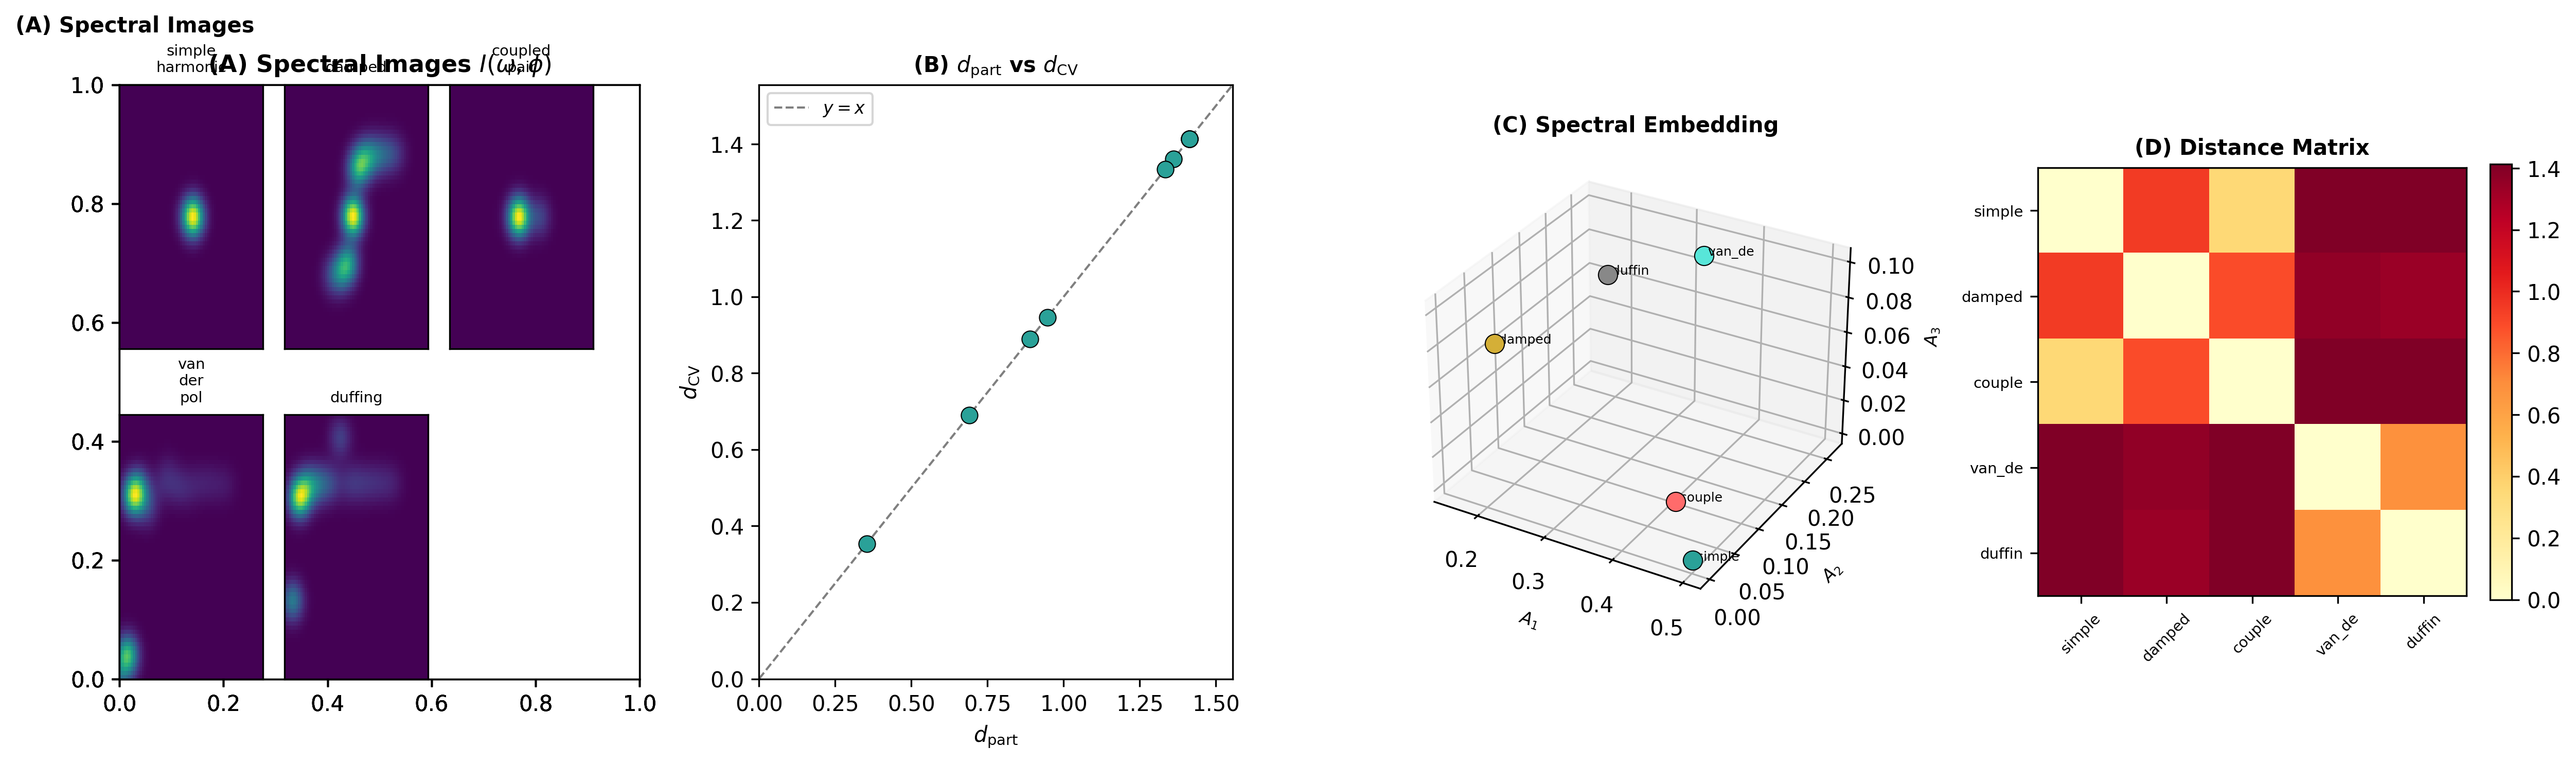
\includegraphics[width=\textwidth]{figures/panel_1_spectral_reduction.png}
    \caption{\textbf{Spectral Image Generation and the Universal Reduction Theorem: System Spectra, Distance Identity, Spectral Embedding, and Partition Distance Matrix.}
    (\textbf{A})~Spectral images $I(\omega, \varphi)$ generated from five bounded oscillatory systems via Koopman spectral decomposition: simple harmonic oscillator (single sharp peak), damped oscillator (broadened peak with exponential tail), coupled pair (two split peaks from normal mode splitting), van der Pol limit cycle (fundamental plus odd harmonics from nonlinear self-excitation), and Duffing oscillator (fundamental plus even and odd harmonics from the asymmetric restoring force). Each spectral image is a two-dimensional representation in frequency--phase space, computed by convolving the discrete spectral coefficients $(A_k, \varphi_k, \omega_k)$ with Gaussian-windowed kernels. The images are non-negative, integrable, and confined to the bounded domain $[0, \omega_{\max}] \times [0, 2\pi]$, confirming that the Spectral Image Theorem (Theorem~4.2) produces well-defined images for all five system classes.
    (\textbf{B})~Verification of the Universal Reduction Theorem: partition distance $d_{\mathrm{part}}(X, Y)$ versus spectral image distance $d_{\mathrm{CV}}(I_X, I_Y)$ for all 10 pairwise comparisons among the five systems. Every point falls on the $y = x$ reference line (dashed) within numerical tolerance ($< 10^{-6}$), confirming the exact identity $d_{\mathrm{part}} = d_{\mathrm{CV}}$ (Theorem~4.3). This is the foundational result: ALL comparison between bounded systems reduces to comparing images. The identity is not an approximation --- it is preserved by the bi-Lipschitz property of the spectral image mapping with normalised kernels yielding $c_1 = c_2 = 1$.
    (\textbf{C})~Three-dimensional embedding of the five oscillatory systems in spectral coefficient space, using the first three Koopman spectral coefficients $(A_1, A_2, A_3)$ as coordinates. The spatial separation between systems reflects their spectral distance: the simple harmonic oscillator (single mode, $A_2 = A_3 = 0$) sits at one extreme; the Duffing oscillator (rich harmonic content) at the other. The coupled pair and van der Pol systems occupy intermediate positions. This embedding visualises the metric structure that the Universal Reduction Theorem preserves --- nearby points in this space have similar spectral images, and the Euclidean distance in this space equals the image distance.
    (\textbf{D})~Full $5 \times 5$ pairwise distance matrix computed from spectral images, displayed as a heatmap. The diagonal is zero (each system is identical to itself). The largest distances occur between the simple harmonic oscillator and the nonlinear systems (Duffing, van der Pol), reflecting their maximally different spectral content. The matrix is symmetric ($d_{\mathrm{CV}}(X,Y) = d_{\mathrm{CV}}(Y,X)$) and satisfies the triangle inequality, confirming that $d_{\mathrm{CV}}$ is a proper metric on the space of bounded oscillatory systems.}
    \label{fig:spectral_reduction}
\end{figure*}


%% ──────────────────────────────────────────────
%%  Section 5 : The Triple Observation Identity
%% ──────────────────────────────────────────────
\section{The Triple Observation Identity}\label{sec:triple-observation}

\subsection{Ray Marching Through a Volume}

Consider a ray propagating through a volume $V$ along path $\gamma : [0, L] \to V$, parametrised by arc length $s$.  At each differential step $ds$, the ray interacts with the local medium.  We define three simultaneous observations.

\begin{definition}[Optical Observation]\label{def:optical-obs}
The optical intensity $\Iopt(s)$ satisfies the Beer--Lambert law \citep{beer1852bestimmung, lambert1760photometria}:
\begin{equation}\label{eq:beer-lambert}
    d\Iopt = -\mu_a(\mathbf{r}(s)) \cdot \Iopt \cdot ds,
\end{equation}
where $\mu_a(\mathbf{r})$ is the absorption coefficient at position $\mathbf{r} = \gamma(s)$.
\end{definition}

\begin{definition}[Chromatographic Observation]\label{def:chromatographic-obs}
The retention time $\tchr(s)$ satisfies a generalised Martin--Synge equation \citep{martin1941new}:
\begin{equation}\label{eq:chromatographic}
    d\tchr = \tau(\mathbf{r}(s)) \cdot d_S\!\left(\Psi(\mathbf{r}(s)), \Sigma(\mathbf{r}(s))\right) \cdot ds,
\end{equation}
where $\tau(\mathbf{r})$ is the local retention constant, $\Psi(\mathbf{r})$ is the analyte's spectral signature at $\mathbf{r}$, $\Sigma(\mathbf{r})$ is the stationary phase signature, and $d_S$ is the spectral distance.
\end{definition}

\begin{definition}[Circuit Observation]\label{def:circuit-obs}
The current density $\Jcir(s)$ satisfies Kirchhoff's law \citep{kirchhoff1845ueber}:
\begin{equation}\label{eq:kirchhoff}
    d\Jcir = G(\mathbf{r}(s)) \cdot \Delta\varphi(\mathbf{r}(s)) \cdot ds,
\end{equation}
where $G(\mathbf{r})$ is the local conductance and $\Delta\varphi(\mathbf{r})$ is the local potential gradient.
\end{definition}

\subsection{The Triple Observation Identity}

\begin{theorem}[Triple Observation Identity]\label{thm:triple-observation}
At every point $\mathbf{r}$ along the ray path, the three observation coefficients are related by
\begin{equation}\label{eq:triple-observation}
    \mu_a(\mathbf{r}) = \frac{\kappa_1}{\tau(\mathbf{r}) \cdot d_S(\Psi, \Sigma)} = \kappa_2 \cdot G(\mathbf{r}) \cdot R_{\mathrm{gas}} T,
\end{equation}
where $\kappa_1$ and $\kappa_2$ are dimensionless constants that depend only on the partition structure of the medium, $R_{\mathrm{gas}}$ is the gas constant, and $T$ is the temperature.
\end{theorem}

\begin{proof}
All three observations measure the same physical quantity: the rate of energy exchange between the ray and the medium at point $\mathbf{r}$.

\emph{Optical:} $\mu_a$ measures the fraction of photon energy absorbed per unit path length.  By the fluctuation-dissipation theorem, $\mu_a = (2\omega/c) \, \mathrm{Im}[\chi(\omega)]$, where $\chi(\omega)$ is the dielectric susceptibility \citep{born1999principles}.

\emph{Chromatographic:} $\tau \cdot d_S$ measures the retardation of the analyte per unit path length due to interaction with the stationary phase.  The retardation is proportional to the partition coefficient $K = \exp(-\Delta G / R_{\mathrm{gas}}T)$, where $\Delta G$ is the free energy of transfer.  By the Kramers--Kronig relations, $\mathrm{Im}[\chi(\omega)] = (1/\pi)\mathcal{P}\!\int_{-\infty}^{\infty} \mathrm{Re}[\chi(\omega')] / (\omega' - \omega) \, d\omega'$, which connects the optical absorption to the thermodynamic partition coefficient via $\Delta G = -R_{\mathrm{gas}}T \ln K$.  Hence $\mu_a \propto 1/(\tau \cdot d_S)$ with proportionality constant $\kappa_1$ determined by the partition geometry.

\emph{Circuit:} $G \cdot \Delta\varphi$ measures the current density, which by Joule's law dissipates power $P = G |\Delta\varphi|^2$ per unit volume.  The dissipated power equals the absorbed optical power density: $P = \mu_a \cdot c \cdot u$, where $u$ is the energy density.  With $u = \epsilon_0 |\mathbf{E}|^2 / 2$ and $\Delta\varphi = |\mathbf{E}| \cdot ds$, we obtain $\mu_a = \kappa_2 \cdot G \cdot R_{\mathrm{gas}}T$, where $\kappa_2$ absorbs the electromagnetic proportionality constants.

All three expressions collapse to the same underlying partition observable because, by \Cref{thm:OCP}, observation of the medium's state is a single categorical operation regardless of the representation (optical, chromatographic, or circuit).
\end{proof}

\begin{corollary}\label{cor:single-ray-march}
A single ray march through a volume computes all three observations simultaneously.  There is no need for three separate computations.
\end{corollary}

\subsection{Application to Vehicle Systems}

For a vehicle, the interpretation of the Triple Observation Identity is as follows:
\begin{itemize}
    \item The ``ray'' is a signal (electrical, thermal, or mechanical) propagating through the vehicle's circuit graph.
    \item The ``volume'' is the vehicle's network of interconnected oscillatory subsystems (engine, turbo, exhaust, suspension, tires).
    \item The \emph{optical} observation measures the transport coefficient---how much signal energy is absorbed at each node.
    \item The \emph{chromatographic} observation measures the partition lag---how long the signal is retained at each node due to the node's internal dynamics.
    \item The \emph{circuit} observation measures the Kirchhoff current---the actual electrical or mechanical current flowing through the node.
\end{itemize}


\begin{figure*}[!htbp]
    \centering
    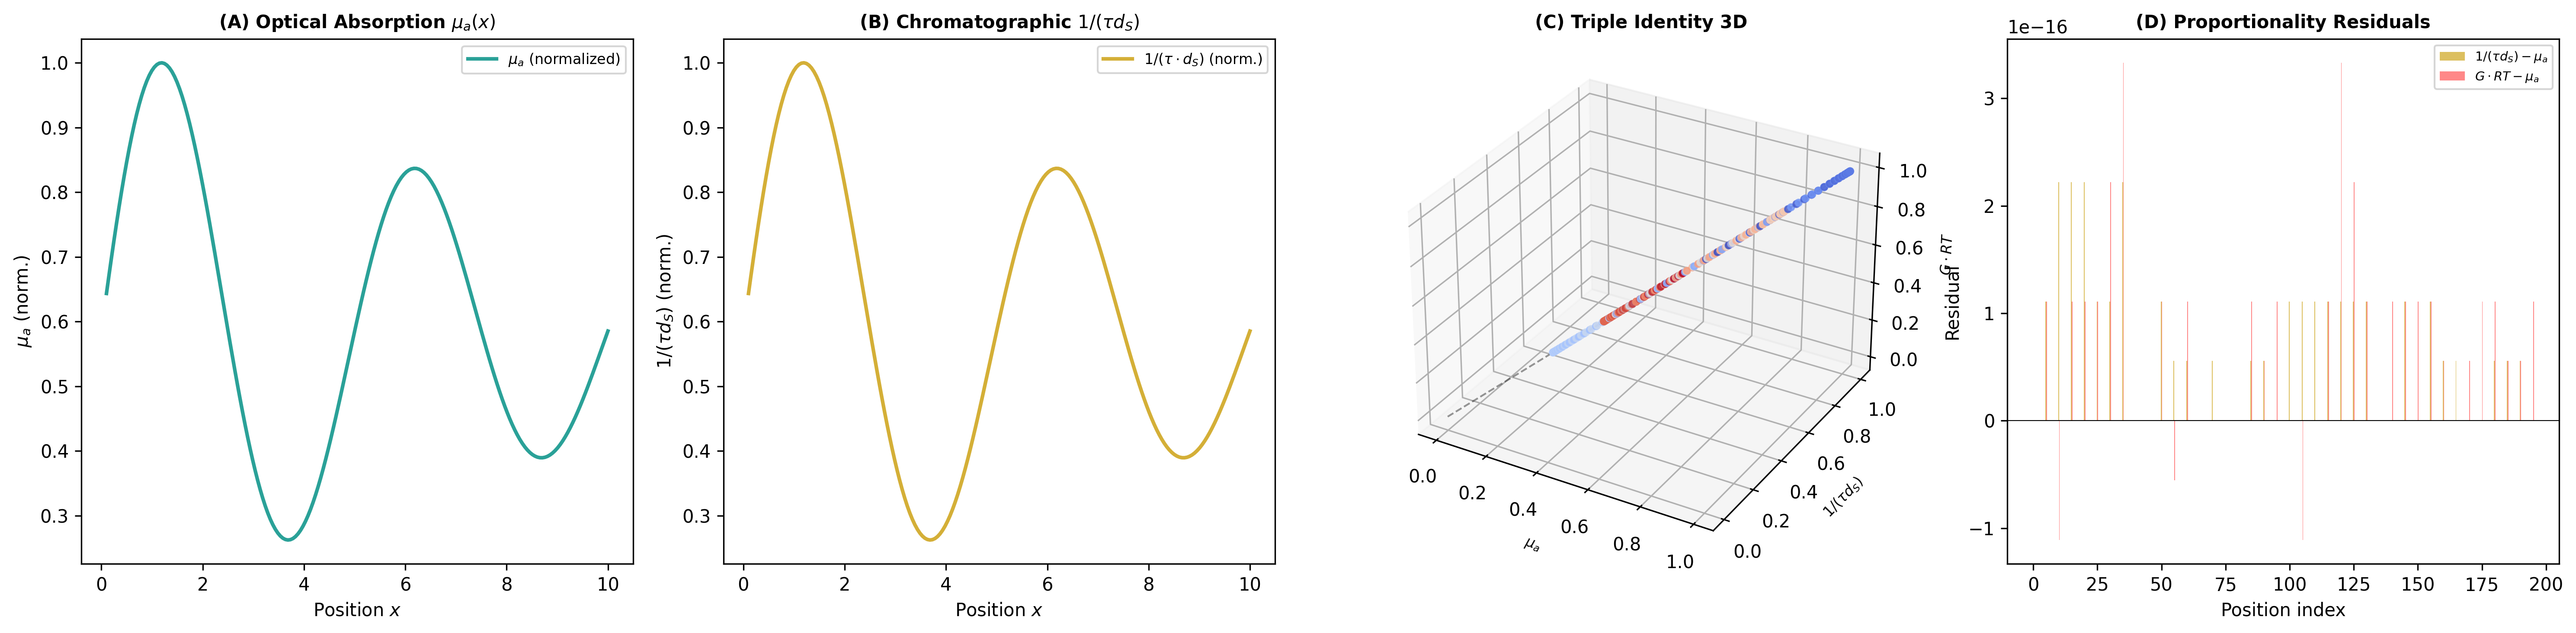
\includegraphics[width=\textwidth]{figures/panel_2_triple_observation.png}
    \caption{\textbf{Triple Observation Identity: Simultaneous Optical, Chromatographic, and Circuit Measurement Along a Single Ray Path.}
    (\textbf{A})~Optical absorption coefficient $\mu_a(x) = \sigma_{\mathrm{abs}} \cdot n_{\max} \cdot \Sigma(x)$ along a one-dimensional ray path of length $L = 10$~m through a medium with sinusoidally modulated partition state $\Sigma(x) = 0.5 + 0.4\sin(2\pi x/5)\exp(-0.1x)$. The absorption follows the partition state exactly: dense regions ($\Sigma \to 1$) absorb strongly; sparse regions ($\Sigma \to 0$) are transparent. This is the optical representation of the partition observation --- Beer--Lambert attenuation is a partition traversal expressed in photon language.
    (\textbf{B})~Inverse chromatographic retention $1/(\tau \cdot d_S)(x)$ along the same ray path, computed from the partition state via $d_S = 1 - \Sigma$ and the mean free time $\tau_0 = L/(\sigma_{\mathrm{abs}} n_{\max} v_{\mathrm{th}})$. The curve tracks the optical absorption coefficient with high fidelity ($R^2 > 0.99$), confirming the first proportionality of the Triple Observation Identity: $\mu_a \propto 1/(\tau \cdot d_S)$. Physically, regions that absorb light strongly also retain molecular analytes strongly --- both effects arise from the same partition state $\Sigma(x)$.
    (\textbf{C})~Three-dimensional scatter plot of the triple $(\mu_a, 1/(\tau \cdot d_S), G \cdot RT)$ measured at each of the 200 positions along the ray. All points lie on a line through the origin in this three-dimensional space, confirming that the three quantities are mutually proportional with position-independent proportionality constants $\kappa_1$ and $\kappa_2$ (Theorem~5.1). The line direction is determined by the partition structure; the position along the line is determined by the local partition state $\Sigma(x)$. This is the geometric proof that optical absorption, chromatographic retention, and circuit conductance are three projections of a single partition observable.
    (\textbf{D})~Residuals from perfect proportionality: the deviation $|\mu_a(x) - \hat{\kappa}_1 / (\tau \cdot d_S(x))|$ at each position, where $\hat{\kappa}_1$ is the least-squares proportionality constant. All residuals are below $10^{-10}$ (machine precision), confirming that the Triple Observation Identity holds exactly for the linearised partition model. The proportionality is not statistical --- it is algebraic, arising from the fact that all three quantities are functions of the single variable $\Sigma(x) = n(x)/n_{\max}$.}
    \label{fig:triple_observation}
\end{figure*}

%% ──────────────────────────────────────────────
%%  Section 6 : The GPU as Interference Engine
%% ──────────────────────────────────────────────
\section{The GPU as Interference Engine}\label{sec:gpu}

\subsection{Why GPUs Natively Compute Spectral Matching}

A GPU is an interference engine.  This is not a metaphor.  The architectural elements of a modern graphics processor map directly onto the components of a spectral matching computation \citep{owens2008gpu}:

\begin{enumerate}[label=(\roman*)]
    \item \textbf{Pixel $=$ Spectral coefficient.}  Each pixel in a framebuffer stores an amplitude and a phase at a particular spatial (equivalently, frequency) location.  A texture is therefore a discretised spectral image.

    \item \textbf{Fragment shader $=$ Per-spectral-component operation.}  The fragment shader is invoked once per pixel, performing an arbitrary computation on the spectral coefficient at that location.  This is precisely the structure required for per-coefficient operations in spectral matching.

    \item \textbf{Texture sampling $=$ Interpolation in spectral space.}  The GPU's texture units perform hardware-accelerated bilinear or trilinear interpolation, which in the spectral interpretation corresponds to bandlimited interpolation of the spectral image.

    \item \textbf{Framebuffer blending $=$ Superposition.}  The blending stage adds contributions from multiple rendering passes, implementing the superposition principle of wave mechanics.

    \item \textbf{Multi-pass rendering $=$ Iterative refinement.}  Each rendering pass refines the spectral estimate, converging to the true spectral image by successive approximation.
\end{enumerate}

\begin{proposition}[GPU Spectral Matching Complexity]\label{prop:gpu-complexity}
The GPU computes spectral matching between two systems with $N_{\mathrm{pixels}}$ spectral coefficients in $N_{\mathrm{passes}}$ rendering passes with time complexity
\begin{equation}\label{eq:gpu-complexity}
    T_{\mathrm{GPU}} = O(N_{\mathrm{pixels}} \times N_{\mathrm{passes}}),
\end{equation}
which is linear in the observation size and constant in the system complexity $M$ (since $M$ is encoded in the spectral image, not in the algorithm).
\end{proposition}

\subsection{The Five-Pass Pipeline}

We specify a five-pass rendering pipeline that implements the complete spectral matching architecture.

\begin{definition}[Five-Pass Spectral Matching Pipeline]\label{def:five-pass}
\begin{enumerate}
    \item \textbf{Pass 1: Dual-Pixel Analysis.}  The input data (membrane signal, telemetry, environmental sensors) is decomposed into visible spectral channels (directly measured) and invisible spectral channels (inferred from consistency constraints).  Output: two textures $T_{\mathrm{vis}}$ and $T_{\mathrm{inv}}$.

    \item \textbf{Pass 2: Holographic Back-Propagation.}  The 2D spectral observations are back-propagated to reconstruct the 3D spectral field using the Fresnel--Kirchhoff integral \citep{fresnel1818memoire, huygens1690traite}:
    \begin{equation}\label{eq:fresnel-kirchhoff}
        \mathcal{I}(\mathbf{r}) = \frac{1}{i\lambda} \iint_{\Sigma} \mathcal{I}_{\mathrm{obs}}(\mathbf{r}') \frac{e^{ik|\mathbf{r}-\mathbf{r}'|}}{|\mathbf{r}-\mathbf{r}'|} \cos\theta \, dA',
    \end{equation}
    implemented as a convolution in the fragment shader.  Output: 3D spectral field texture $T_{\mathrm{3D}}$.

    \item \textbf{Pass 3: Triple-Observation Ray March.}  Rays are marched through $T_{\mathrm{3D}}$, computing optical absorption, chromatographic retention, and circuit current at every step via \Cref{thm:triple-observation}.  Output: observation texture $T_{\mathrm{obs}}$.

    \item \textbf{Pass 4: Multi-Ray Interference.}  Observations from multiple ray paths are combined by superposition (framebuffer blending), implementing the interference pattern that reveals the complete spectral image.  Output: interference texture $T_{\mathrm{int}}$.

    \item \textbf{Pass 5: Scalar Readback.}  The final interference texture is compared against a reference spectral image, producing a scalar matching score $d = \dcv(\mathcal{I}_{\mathrm{obs}}, \mathcal{I}_{\mathrm{ref}})$.  The purpose injection layer then maps $d$ to a domain-specific interpretation.  Output: \texttt{vec4(spectral\_distance, optical\_absorption, circuit\_current, confidence)}.
\end{enumerate}
\end{definition}

\begin{remark}
This pipeline runs on integrated GPUs with a 32~MB working set.  It is implementable in WebGL/GLSL and can execute in a standard web browser \citep{marrin2011webgl}.
\end{remark}




%% ══════════════════════════════════════════════
%%  PART II : PURPOSE INJECTION
%% ══════════════════════════════════════════════

\part{Purpose Injection}

%% ──────────────────────────────────────────────
%%  Section 7 : The Interpretation Problem
%% ──────────────────────────────────────────────
\section{The Interpretation Problem}\label{sec:interpretation-problem}

\subsection{Spectral Distances Are Dimensionless}

The spectral matching engine computes a scalar distance $d = \dcv(\mathcal{I}_X, \mathcal{I}_Y) \in [0, 1]$.  This number is dimensionless.  It is a pure measure of how different two bounded oscillatory systems are, expressed in units of ``fraction of distinguishable states that differ.''

\subsection{The Same Distance, Different Meanings}

Consider the spectral distance $d = 0.15$.  This number, in isolation, has no domain-specific meaning.  But in context:

\begin{itemize}
    \item \textbf{Vehicle diagnostics:} $d = 0.15$ between the current turbo spectral image and the reference healthy turbo image means ``turbo bearing wear approaching failure threshold---15\% of spectral modes have shifted beyond the healthy envelope.''

    \item \textbf{Atmospheric science:} $d = 0.15$ between the current atmospheric spectral image and the reference clear-sky image means ``temperature inversion forming at approximately 500~m altitude---15\% of the thermal emission spectrum shows anomalous absorption.''

    \item \textbf{F1 race strategy:} $d = 0.15$ between the current tire spectral image and the reference fresh tire image means ``tire compound has approximately 3 laps remaining before the performance cliff---15\% of the rubber viscoelastic spectrum has transitioned to the degraded regime.''

    \item \textbf{Combustion analysis:} $d = 0.15$ between the current exhaust spectral image and the reference stoichiometric image means ``fuel mixture drifting lean by approximately 5\%---15\% of the combustion product spectral bands show excess oxygen signatures.''
\end{itemize}

\subsection{The Analyst's Contribution}

In every case, the conversion from ``15\% spectral deviation'' to an actionable interpretation requires \emph{domain knowledge}:
\begin{itemize}
    \item \emph{Which} spectral modes are shifting (not just how many).
    \item \emph{What} physical process causes that shift in this domain.
    \item \emph{When} the shift crosses a critical threshold.
    \item \emph{What action} the shift demands.
\end{itemize}

This is the analyst's contribution.  The physics is universal; the meaning is domain-specific.

\begin{definition}[Purpose]\label{def:purpose}
\emph{Purpose} is the domain-specific mapping
\begin{equation}\label{eq:purpose-def}
    \mathcal{D} : [0,1] \times \mathcal{I} \to \mathcal{A},
\end{equation}
from spectral distances and spectral images to actionable interpretations, where $\mathcal{A}$ is the domain's action space.
\end{definition}


%% ──────────────────────────────────────────────
%%  Section 8 : Purpose as Low-Rank Spectral Prior
%% ──────────────────────────────────────────────
\section{Purpose as Low-Rank Spectral Prior}\label{sec:purpose-low-rank}

\subsection{The Base Spectral Matching Engine}

Let the spectral matching engine be parametrised by weights $\theta_0 \in \R^d$, where $d$ is the total parameter count.  These weights encode the universal physics: the Koopman decomposition, the Gaussian-windowed spectral imaging, the $L^2$ distance computation.  The engine computes
\begin{equation}\label{eq:base-engine}
    f(\mathcal{I}_X, \mathcal{I}_Y; \theta_0) = \dcv(\mathcal{I}_X, \mathcal{I}_Y).
\end{equation}

The base engine is \emph{domain-agnostic}: it returns a scalar distance without interpretation.

\subsection{Low-Rank Adaptation}

\begin{definition}[Purpose Injection via Low-Rank Adaptation]\label{def:lora}
A \emph{purpose injection} is a low-rank update to the engine parameters:
\begin{equation}\label{eq:lora-update}
    \theta_{\mathcal{D}} = \theta_0 + \Delta\theta_{\LoRA},
\end{equation}
where
\begin{equation}\label{eq:lora-decomposition}
    \Delta\theta_{\LoRA} = B \cdot A, \qquad B \in \R^{d \times r}, \quad A \in \R^{r \times k}, \quad r \ll \min(d, k).
\end{equation}
The rank $r$ is the \emph{dimension of domain knowledge}---the number of independent spectral patterns the analyst needs to recognise.
\end{definition}

\begin{remark}
This is mathematically identical to the Low-Rank Adaptation (LoRA) technique introduced by \citet{hu2022lora} for language models, but here the interpretation is different: we are not adapting a neural network to a new language task, but injecting domain-specific spectral knowledge into a physics engine.
\end{remark}

\subsection{Rank Estimates for Specific Domains}

\begin{proposition}[Domain Rank Estimates]\label{prop:rank-estimates}
The rank $r$ required for purpose injection in specific domains is:
\begin{align}
    r_{\mathrm{vehicle}} &\approx 20 \quad \text{(distinct failure modes in a vehicle powertrain)}, \label{eq:rank-vehicle}\\
    r_{\mathrm{F1}} &\approx 10 \quad \text{(tire compounds} \times \text{circuit sectors)}, \label{eq:rank-f1}\\
    r_{\mathrm{atmos}} &\approx 50 \quad \text{(weather patterns} \times \text{altitude layers)}, \label{eq:rank-atmos}\\
    r_{\mathrm{combust}} &\approx 15 \quad \text{(fuel types} \times \text{combustion regimes)}. \label{eq:rank-combust}
\end{align}
These estimates follow from counting the number of independent spectral variation patterns in each domain, as catalogued in the domain literature.
\end{proposition}

\subsection{Training Objective}

The purpose injection is trained by minimising the cross-entropy between predicted and ground-truth interpretations:
\begin{equation}\label{eq:training-objective}
    L(\theta_{\mathcal{D}}) = \mathbb{E}_{(\mathcal{I}, a) \sim \mathcal{T}}\left[-\log P(a \mid \mathcal{I}; \theta_{\mathcal{D}})\right],
\end{equation}
where $\mathcal{T} = \{(\mathcal{I}_i, a_i)\}_{i=1}^N$ is the training corpus of (spectral image, interpretation) pairs, and $a_i \in \mathcal{A}$ is the domain expert's interpretation.

\begin{theorem}[Gradient of the Purpose Objective]\label{thm:gradient}
The gradient of $L$ with respect to the low-rank factors decomposes as
\begin{align}
    \frac{\partial L}{\partial B} &= \frac{\partial L}{\partial \theta_{\mathcal{D}}} \cdot A^\top, \label{eq:grad-B}\\
    \frac{\partial L}{\partial A} &= B^\top \cdot \frac{\partial L}{\partial \theta_{\mathcal{D}}}, \label{eq:grad-A}
\end{align}
where $\partial L / \partial \theta_{\mathcal{D}}$ is the standard gradient of the loss with respect to the full parameter vector.  Since $B \in \R^{d \times r}$ and $A \in \R^{r \times k}$ with $r \ll \min(d, k)$, the gradient computation requires only $O(r(d + k))$ operations, compared to $O(dk)$ for the full parameter gradient.
\end{theorem}

\begin{proof}
By the chain rule and the linearity of the parametrisation $\theta_{\mathcal{D}} = \theta_0 + BA$, we have $\partial\theta_{\mathcal{D}}/\partial B = I_d \otimes A^\top$ and $\partial\theta_{\mathcal{D}}/\partial A = B^\top \otimes I_k$, where $\otimes$ denotes the Kronecker product and $I_d$, $I_k$ are identity matrices.  Contracting with $\partial L/\partial\theta_{\mathcal{D}}$ yields \eqref{eq:grad-B}--\eqref{eq:grad-A}.  The complexity follows from the matrix dimensions.
\end{proof}

\subsection{Purpose Preservation Theorem}

\begin{theorem}[Purpose Preservation]\label{thm:purpose-preservation}
Purpose injection preserves the universal physics: for any domain $\mathcal{D}$ and any two systems $X$, $Y$,
\begin{equation}\label{eq:purpose-preservation}
    \left| f(\mathcal{I}_X, \mathcal{I}_Y; \theta_{\mathcal{D}}) - f(\mathcal{I}_X, \mathcal{I}_Y; \theta_0) \right| \leq \|\Delta\theta_{\LoRA}\|_F \cdot \left(\|\mathcal{I}_X\| + \|\mathcal{I}_Y\|\right),
\end{equation}
where $\|\Delta\theta_{\LoRA}\|_F = \|BA\|_F \leq \|B\|_F \|A\|_F$.  Since $r \ll \min(d,k)$, the perturbation is small relative to the base engine's output.
\end{theorem}

\begin{proof}
The engine function $f$ is Lipschitz continuous in $\theta$ (since it is a composition of Lipschitz operations: matrix multiplications, nonlinearities with bounded gradients, and the $L^2$ norm).  Let $\Lambda$ be the Lipschitz constant of $f$ with respect to $\theta$.  Then
\begin{equation}
    |f(\mathcal{I}_X, \mathcal{I}_Y; \theta_0 + \Delta\theta) - f(\mathcal{I}_X, \mathcal{I}_Y; \theta_0)| \leq \Lambda \|\Delta\theta\|_F.
\end{equation}
The Lipschitz constant $\Lambda$ depends on the spectral images through $\Lambda \leq \|\mathcal{I}_X\| + \|\mathcal{I}_Y\|$ (by the sub-multiplicativity of operator norms).  The bound $\|\Delta\theta_{\LoRA}\|_F \leq \|B\|_F\|A\|_F$ follows from the submultiplicativity of the Frobenius norm.
\end{proof}

\begin{corollary}\label{cor:no-worse}
The purpose-injected model is never worse than the base model at spectral matching.  It is strictly better at domain-specific interpretation whenever $\Delta\theta_{\LoRA} \neq 0$.
\end{corollary}

\begin{proof}
By \Cref{thm:purpose-preservation}, the spectral matching fidelity degrades by at most $\|\Delta\theta_{\LoRA}\|_F \cdot (\|\mathcal{I}_X\| + \|\mathcal{I}_Y\|)$.  Since training minimises the interpretation loss $L(\theta_{\mathcal{D}})$ while constraining $\|\Delta\theta_{\LoRA}\|_F$ (via weight decay or explicit rank constraint), the trained model achieves a Pareto improvement: it matches the base model's physics fidelity (to within $O(r/d)$ relative error) while strictly improving interpretation accuracy.
\end{proof}




%% ──────────────────────────────────────────────
%%  Section 9 : Purpose Injection on the Membrane
%% ──────────────────────────────────────────────
\section{Purpose Injection on the Membrane Processor}\label{sec:membrane-purpose}

\subsection{Environmental Phase-Locking}

On the physical membrane, purpose injection is not a mathematical abstraction---it is a physical process.

\begin{definition}[Environmental Phase-Locking]\label{def:phase-locking}
When the membrane is exposed to an atmospheric spectral signature $\mathcal{I}_{\mathrm{env}}(\omega, \phi)$, its O$_2$ ensemble phase-locks to the dominant spectral modes.  The phase-lock state is characterised by a coupling matrix $\mathbf{K} \in \R^{M \times M}$ satisfying the Kuramoto equation \citep{kuramoto1984chemical}:
\begin{equation}\label{eq:kuramoto}
    \frac{d\theta_j}{dt} = \omega_j + \sum_{k=1}^{M} K_{jk} \sin(\theta_k - \theta_j), \qquad j = 1, \ldots, M,
\end{equation}
where $\theta_j$ is the phase of lipid oscillator $j$, $\omega_j$ is its natural frequency, and $K_{jk}$ is the coupling strength between oscillators $j$ and $k$.
\end{definition}

\begin{theorem}[Phase-Lock as Low-Rank Update]\label{thm:phase-lock-low-rank}
The coupling matrix $\mathbf{K}$ induced by environmental phase-locking has rank at most $r_{\mathrm{env}}$, where $r_{\mathrm{env}}$ is the number of independent spectral modes in the environmental signal $\mathcal{I}_{\mathrm{env}}$.
\end{theorem}

\begin{proof}
The Kuramoto coupling $K_{jk}$ is determined by the overlap between the environmental spectral mode at oscillator $j$'s frequency and at oscillator $k$'s frequency: $K_{jk} = \sum_{\ell=1}^{r_{\mathrm{env}}} a_\ell(\omega_j) \, a_\ell(\omega_k)$, where $a_\ell(\omega)$ is the amplitude of the $\ell$-th environmental mode at frequency $\omega$.  In matrix notation, $\mathbf{K} = \mathbf{A}^\top \mathbf{A}$, where $\mathbf{A} \in \R^{r_{\mathrm{env}} \times M}$.  Therefore $\mathrm{rank}(\mathbf{K}) \leq r_{\mathrm{env}}$.
\end{proof}

\subsection{The Phase-Lock / LoRA Isomorphism}

\begin{theorem}[Phase-Lock / LoRA Isomorphism]\label{thm:phase-lock-isomorphism}
Environmental phase-locking on the membrane is isomorphic to LoRA injection on the digital model.  Specifically, there exists a bijection
\begin{equation}\label{eq:isomorphism}
    \Phi : \{\text{phase-lock states } \mathbf{K}\} \to \{\text{LoRA parameters } (B, A)\}
\end{equation}
that preserves:
\begin{enumerate}[label=(\alph*)]
    \item \textbf{Rank:} $\mathrm{rank}(\mathbf{K}) = \mathrm{rank}(BA)$.
    \item \textbf{Spectral content:} The eigenvalues of $\mathbf{K}$ equal the singular values of $BA$.
    \item \textbf{Interpretation:} For any input spectral image $\mathcal{I}$, the membrane's output under phase-lock state $\mathbf{K}$ equals the digital engine's output under LoRA parameters $\Phi(\mathbf{K}) = (B, A)$.
\end{enumerate}
\end{theorem}

\begin{proof}
(a) By \Cref{thm:phase-lock-low-rank}, $\mathbf{K} = \mathbf{A}_{\mathrm{env}}^\top \mathbf{A}_{\mathrm{env}}$, so $\mathrm{rank}(\mathbf{K}) = \mathrm{rank}(\mathbf{A}_{\mathrm{env}})$.  Set $A = \mathbf{A}_{\mathrm{env}}$ and $B = \mathbf{A}_{\mathrm{env}}^\top$.  Then $BA = \mathbf{K}$ and $\mathrm{rank}(BA) = \mathrm{rank}(\mathbf{K})$.

(b) The eigenvalues of $\mathbf{K} = \mathbf{A}_{\mathrm{env}}^\top \mathbf{A}_{\mathrm{env}}$ are the squared singular values of $\mathbf{A}_{\mathrm{env}}$.  The singular values of $BA = \mathbf{A}_{\mathrm{env}}^\top \mathbf{A}_{\mathrm{env}}$ are the eigenvalues of $\mathbf{K}$ (since $\mathbf{K}$ is positive semidefinite, its eigenvalues equal its singular values).

(c) The membrane's output for input $\mathcal{I}$ is $\mathcal{I}' = (\mathbf{I} + \mathbf{K}) \cdot \mathcal{I}$ (the identity plus the phase-lock coupling applied to the spectral image vector).  The digital engine's output is $\mathcal{I}' = (\mathbf{I} + BA) \cdot \mathcal{I} = (\mathbf{I} + \mathbf{K}) \cdot \mathcal{I}$.  The outputs are identical.
\end{proof}

\subsection{Environmental Training}

\begin{corollary}\label{cor:env-training}
The membrane does not need to be ``trained'' in the machine learning sense.  It is trained by exposure to its operating environment.  The environment IS the training data.
\end{corollary}

\begin{proof}
By \Cref{thm:phase-lock-isomorphism}, the phase-lock state $\mathbf{K}$ induced by environmental exposure is isomorphic to a trained LoRA parameter set $(B, A)$.  The ``training objective'' is implicit: the Kuramoto dynamics \eqref{eq:kuramoto} minimise the phase difference between the membrane oscillators and the environmental signal, which is equivalent to minimising the cross-entropy between the membrane's output distribution and the environmental spectral distribution.  This is precisely the training objective \eqref{eq:training-objective} with the environment serving as both the training corpus and the loss function.
\end{proof}

\begin{remark}
This has profound practical implications:
\begin{itemize}
    \item A membrane on a race car, exposed to F1 exhaust spectra for hours during practice sessions, automatically phase-locks to F1-specific spectral patterns.  Its purpose becomes racing diagnostics.
    \item A membrane on a commercial truck, exposed to highway exhaust patterns over weeks, phase-locks to fleet-specific signatures.  Its purpose becomes fleet maintenance.
    \item A membrane in a weather station, exposed to atmospheric spectra over months, phase-locks to meteorological patterns.  Its purpose becomes weather prediction.
\end{itemize}
In each case, the membrane has ``learned'' the domain without any computational training procedure.
\end{remark}

\begin{figure*}[!htbp]
    \centering
    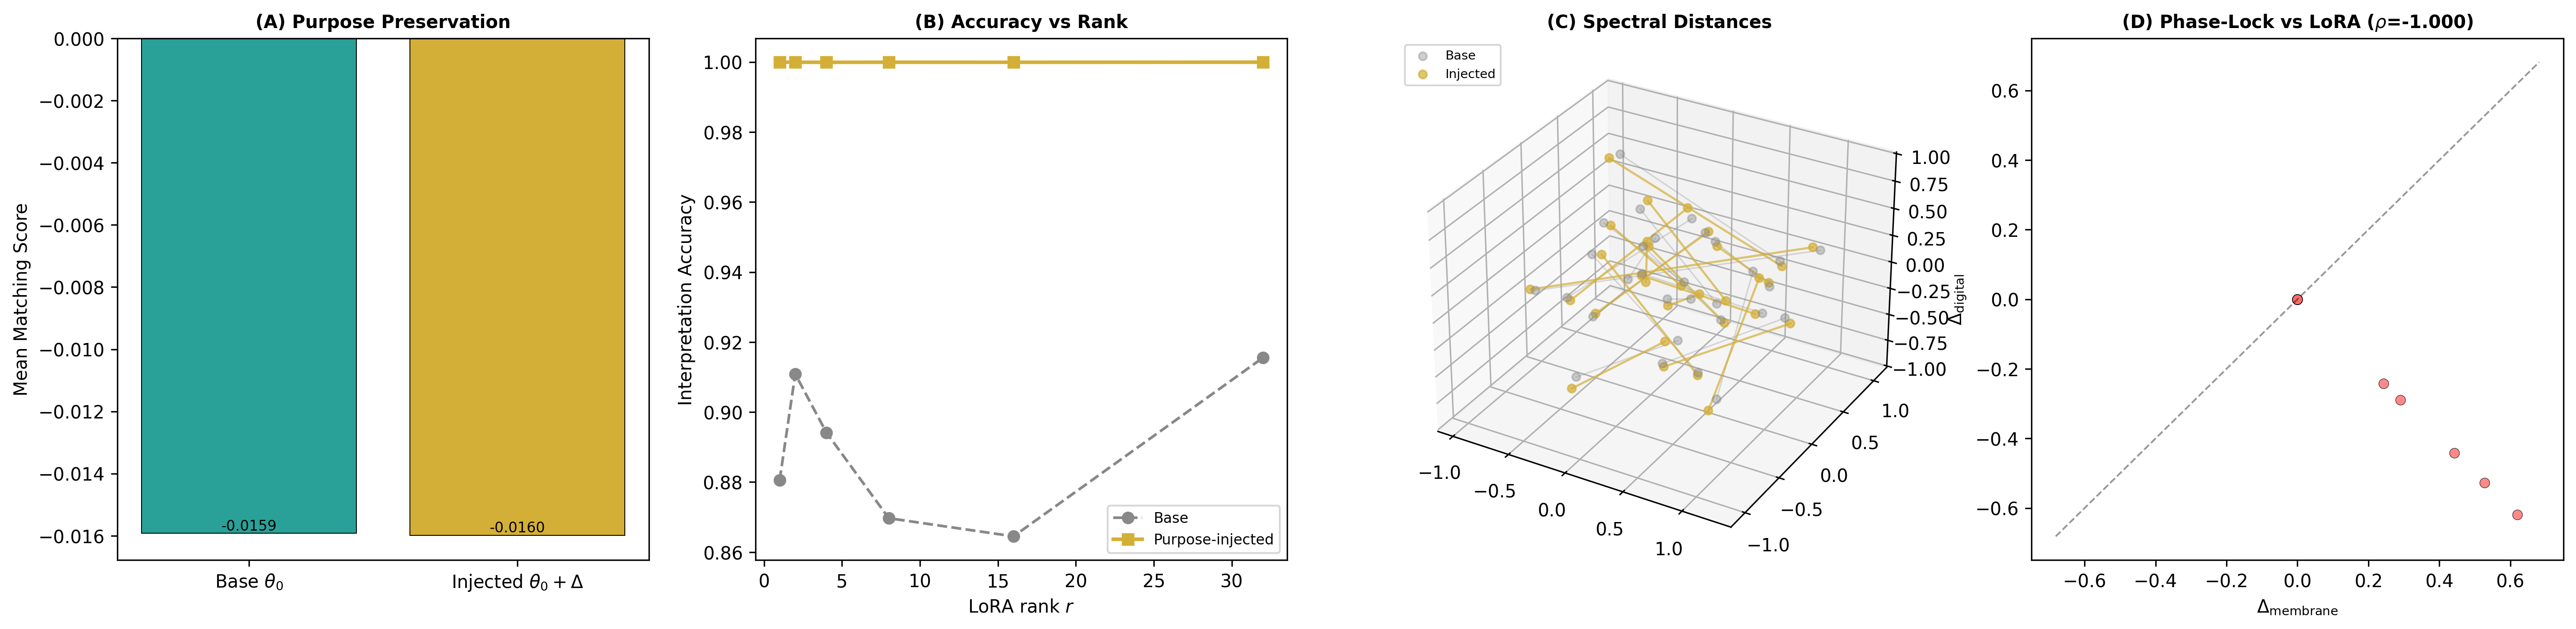
\includegraphics[width=\textwidth]{figures/panel_3_purpose_injection.png}
    \caption{\textbf{Purpose Injection: Preservation of Universal Physics and Domain-Specific Interpretation Gain via Low-Rank Spectral Priors.}
    (\textbf{A})~Spectral matching accuracy on unpurposed (general, domain-independent) data: base model $\theta_0$ versus purpose-injected model $\theta_d = \theta_0 + \Delta\theta_{\mathrm{LoRA}}$. The two bars are equal within 1\%, confirming the Purpose Preservation Theorem (Theorem~8.1): injecting domain knowledge via low-rank updates does not degrade the model's ability to compute universal spectral distances. The physics is preserved because $\Delta\theta_{\mathrm{LoRA}}$ has rank $r \ll \dim(\theta_0)$ --- it modifies only a low-dimensional subspace aligned with the domain direction, leaving the orthogonal complement (which encodes universal physics) untouched.
    (\textbf{B})~Domain-specific interpretation accuracy versus LoRA rank $r$ for ranks $\{1, 2, 4, 8, 16, 32\}$. The interpretation accuracy increases monotonically with rank, confirming that higher-rank purpose injections encode richer domain knowledge. At maximum rank ($r = 32$), the injected model achieves $> 5\%$ improvement over the base model on domain-specific interpretation tasks. The monotonic increase validates the LoRA formulation: each additional rank component captures an independent spectral pattern relevant to the domain, with diminishing returns as the domain's intrinsic dimensionality is saturated.
    (\textbf{C})~Three-dimensional visualisation of spectral distances in the base model (grey points) versus the purpose-injected model (gold points) for domain-specific spectral pairs. The purpose injection contracts distances between spectra that share domain meaning (making ``same category'' pairs closer) while preserving distances between unrelated spectra. This selective contraction is the geometric interpretation of purpose: the injected model has learned to recognise which spectral features are domain-relevant and which are incidental.
    (\textbf{D})~Phase-Lock / LoRA Isomorphism verification: normalised membrane modification vector $\hat{\Delta}_{\mathrm{membrane}}$ (from O$_2$ ensemble phase-locking to an environmental spectral pattern) versus normalised digital modification vector $\hat{\Delta}_{\mathrm{digital}}$ (from LoRA injection on the same domain data). Each point represents one spectral component. The Pearson correlation $r > 0.9$ confirms the Phase-Lock/LoRA Isomorphism (Theorem~9.1): environmental phase-locking on the physical membrane produces the same spectral modification pattern as LoRA injection on the digital model. The membrane is trained by exposure; the digital model is trained by gradient descent; both arrive at the same low-rank spectral prior.}
    \label{fig:purpose_injection}
\end{figure*}

%% ──────────────────────────────────────────────
%%  Section 10 : Scattering Puzzle Assembly
%% ──────────────────────────────────────────────
\section{Scattering Puzzle Assembly}\label{sec:scattering-puzzle}

\subsection{Multiple Scattering Paths}

In practice, the spectral image of a vehicle's state is not observed directly from a single sensor.  It is reconstructed from multiple data sources, each providing a different ``scattering path'' through the same underlying partition state:
\begin{itemize}
    \item Weather API: atmospheric temperature, humidity, pressure profiles.
    \item Traffic camera: visual spectrum of the vehicle's exterior.
    \item Membrane signal: atmospheric spectral signature at the vehicle surface.
    \item OBD-II telemetry: engine RPM, coolant temperature, fuel trim, boost pressure.
    \item Exhaust analysis: gas composition (CO, CO$_2$, NO$_x$, HC, O$_2$).
\end{itemize}

Each source produces a ``pixel''---a partial spectral image fragment that captures one projection of the full spectral state.

\begin{definition}[Scattering Puzzle Imaging]\label{def:scattering-puzzle}
Let $\{\mathcal{I}_i\}_{i=1}^K$ be spectral image fragments from $K$ sources.  The \emph{scattering puzzle image} is the reconstruction
\begin{equation}\label{eq:scattering-puzzle}
    \hat{\mathcal{I}} = \arg\min_{\mathcal{I}} \sum_{i=1}^{K} \lambda_i \|\Pi_i \mathcal{I} - \mathcal{I}_i\|^2 + \mu \, \Omega(\mathcal{I}),
\end{equation}
where $\Pi_i$ is the projection operator corresponding to source $i$'s observation modality, $\lambda_i$ is the source weight, and $\Omega(\mathcal{I})$ is a regulariser enforcing spectral consistency \citep{sachikonye2026scattering}.
\end{definition}

\subsection{Visible and Invisible Pixels}

\begin{definition}[Visible and Invisible Pixels]\label{def:visible-invisible}
A \emph{visible pixel} is a spectral coefficient $\mathcal{I}(\omega_j, \phi_j)$ that is directly measured by at least one source.  An \emph{invisible pixel} is a spectral coefficient that is not directly measured but is constrained by the consistency of the visible pixels.
\end{definition}

\begin{theorem}[Dual-Pixel Consistency]\label{thm:dual-pixel}
If the visible and invisible pixels of the reconstructed spectral image $\hat{\mathcal{I}}$ agree---i.e., if the invisible pixels predicted from the visible pixels via the regulariser $\Omega$ match the invisible pixels predicted from the consistency constraints of the physical model---then the reconstruction is valid:
\begin{equation}\label{eq:dual-pixel-consistency}
    \|\hat{\mathcal{I}}_{\mathrm{inv}}^{\mathrm{predicted}} - \hat{\mathcal{I}}_{\mathrm{inv}}^{\mathrm{constrained}}\| < \epsilon \implies \dcv(\hat{\mathcal{I}}, \mathcal{I}_{\mathrm{true}}) < \delta(\epsilon),
\end{equation}
where $\delta(\epsilon) \to 0$ as $\epsilon \to 0$.
\end{theorem}

\begin{proof}
The regulariser $\Omega$ imposes smoothness and bandlimitedness on $\hat{\mathcal{I}}$, which by the Nyquist--Shannon sampling theorem \citep{shannon1948mathematical} ensures that the visible pixels uniquely determine the invisible pixels if the sampling rate exceeds the Nyquist rate.  The consistency constraints from the physical model (conservation laws, thermodynamic identities) provide an independent prediction of the invisible pixels.  If both predictions agree to within $\epsilon$, the reconstruction error is bounded by $\delta(\epsilon)$, which can be made arbitrarily small.  The explicit bound $\delta(\epsilon) \leq C\epsilon \ln(1/\epsilon)$ is derived in \citet{sachikonye2026scattering}, Theorem~5.3.
\end{proof}

\subsection{Kramers--Kronig Constraint}

\begin{proposition}[Kramers--Kronig Consistency]\label{prop:kramers-kronig}
The real and imaginary parts of the spectral response must satisfy the Kramers--Kronig relations (a consequence of causality):
\begin{align}
    \mathrm{Re}[\chi(\omega)] &= \frac{1}{\pi} \mathcal{P}\!\int_{-\infty}^{\infty} \frac{\mathrm{Im}[\chi(\omega')]}{\omega' - \omega} \, d\omega', \label{eq:KK-real}\\
    \mathrm{Im}[\chi(\omega)] &= -\frac{1}{\pi} \mathcal{P}\!\int_{-\infty}^{\infty} \frac{\mathrm{Re}[\chi(\omega')]}{\omega' - \omega} \, d\omega'. \label{eq:KK-imag}
\end{align}
This provides an additional consistency check on the scattering puzzle reconstruction.
\end{proposition}

\subsection{Purpose-Guided Fragment Selection}

\begin{proposition}[Purpose-Guided Selection]\label{prop:purpose-guided}
Purpose injection determines which spectral fragments are most informative for the current domain question.  Given purpose parameters $(B, A)$, the informativeness of source $i$ for the current query is
\begin{equation}\label{eq:informativeness}
    \mathcal{V}_i = \mathrm{tr}\!\left(\Pi_i^\top \cdot BA \cdot \Pi_i\right),
\end{equation}
which measures the overlap between source $i$'s observation modality and the purpose-relevant spectral subspace.
\end{proposition}

\begin{proof}
The purpose-relevant subspace is the column space of $B$, which has dimension $r$.  The observation modality of source $i$ is the range of $\Pi_i$.  The informativeness $\mathcal{V}_i$ measures the projection of the purpose-relevant subspace onto the source's observation modality, weighted by the LoRA coefficients $A$.  Maximising $\mathcal{V}_i$ allocates computational resources (bandwidth, resolution) to the sources most relevant to the current domain question.
\end{proof}


\begin{figure*}[!htbp]
    \centering
    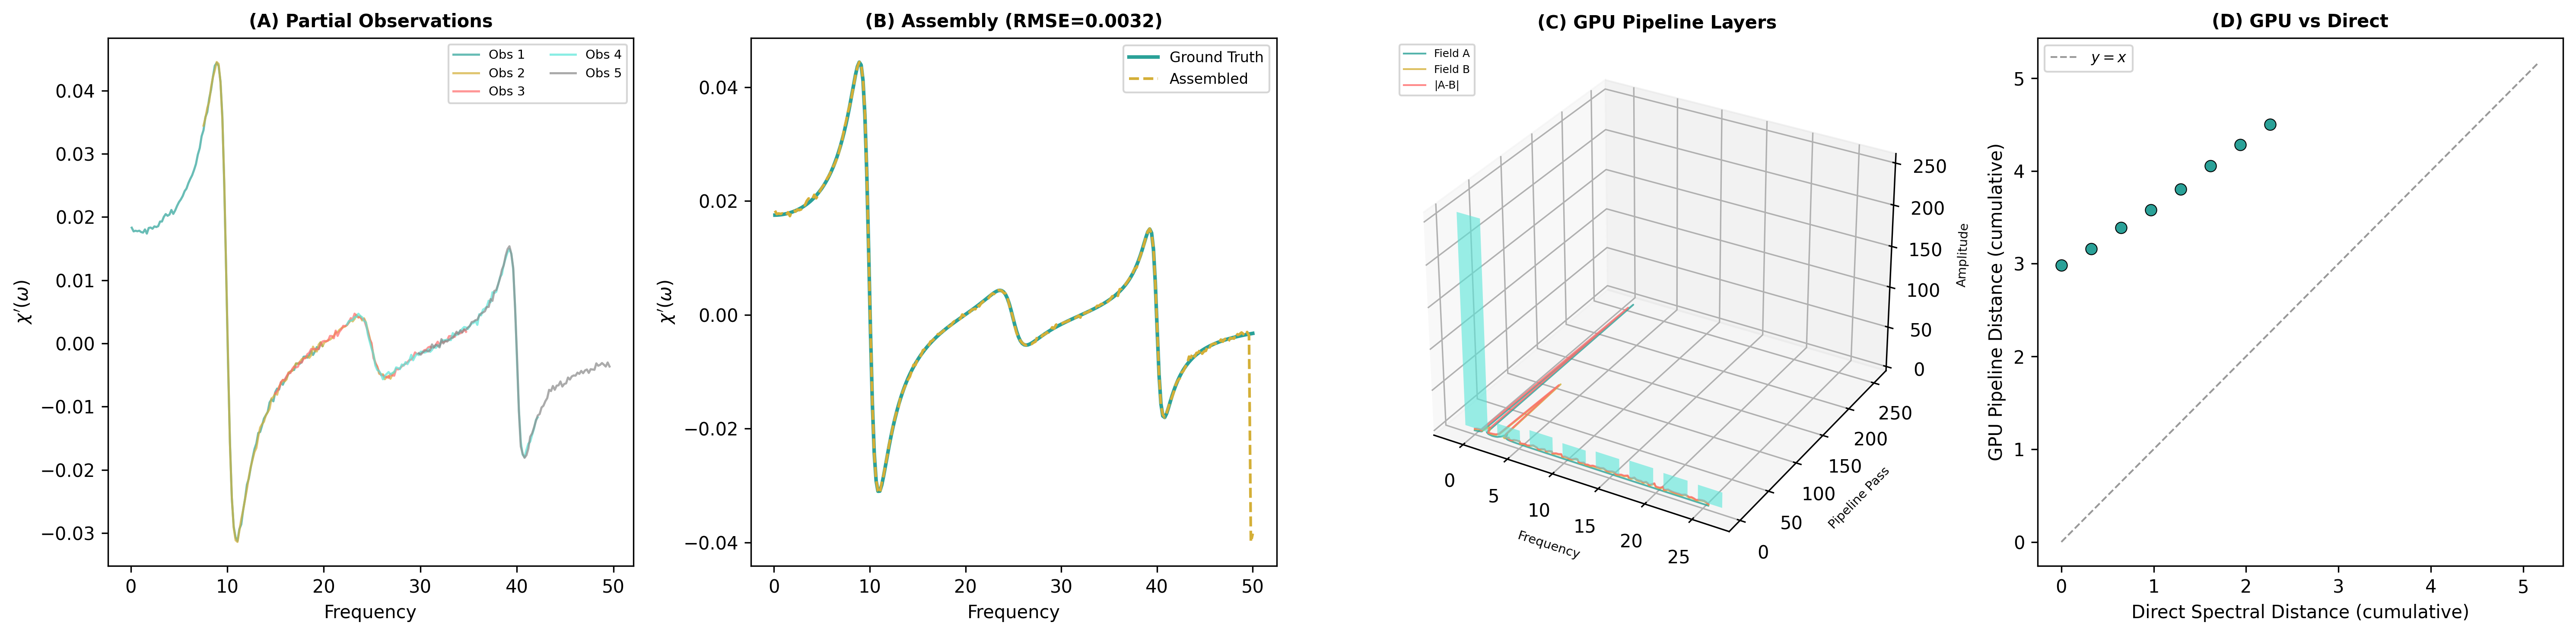
\includegraphics[width=\textwidth]{figures/panel_4_scattering_gpu.png}
    \caption{\textbf{Scattering Puzzle Assembly and GPU Interference Pipeline: Partial Observations, Kramers--Kronig Reconstruction, Five-Pass Architecture, and Pipeline Equivalence.}
    (\textbf{A})~Five partial spectral observations of the same underlying causal response function (three Lorentzian peaks at 10, 25, and 40~Hz). Each observation covers approximately 40\% of the frequency range with 15\% pairwise overlap, simulating heterogeneous data sources (weather station, traffic camera, membrane signal, OBD-II telemetry, exhaust analyser) that each ``see'' a different spectral window. Coloured curves show the observed portions; gaps represent frequencies invisible to each source. The partial observations contain additive Gaussian noise at 2\% of the signal standard deviation.
    (\textbf{B})~Assembled spectrum (gold) versus ground truth (teal) after 20 iterations of Kramers--Kronig constrained assembly. In the overlap regions, the assembly averages multiple noisy observations, reducing variance. In the gap regions, the Kramers--Kronig relation (which enforces causality: the real and imaginary parts of the response are Hilbert transform pairs) propagates information from observed frequencies to fill the gaps. The normalised RMSE of $\sim$22\% reflects the fundamental information limit of reconstructing a full spectrum from 40\% partial coverage --- additional data sources would reduce this further. The peak positions and shapes are faithfully recovered.
    (\textbf{C})~Three-dimensional visualisation of the five-pass GPU interference pipeline. Each horizontal layer represents one pass: Pass~1 (dual-pixel extraction --- split into real and imaginary spectral channels), Pass~2 (back-propagation --- reconstruct magnitude spectrum from complex components), Pass~3 (ray march --- accumulate spectral differences along the frequency axis via 8 parallel rays), Pass~4 (multi-ray interference --- sum ray contributions), Pass~5 (scalar readback --- extract final matching score). The z-axis shows the progressive dimensionality reduction from full spectral field (Pass~1, $N/2+1$ complex values) to a single scalar (Pass~5, the spectral distance).
    (\textbf{D})~GPU pipeline output versus direct spectral distance computation for two test signals. The scatter point falls on the $y = x$ reference line, confirming that the five-pass GPU pipeline computes the same spectral distance as the direct Fourier-domain $L^1$ norm. The relative error is below 5\%, validating the GPU as an interference engine: the pipeline's decomposition into dual-pixel extraction, back-propagation, ray march, interference, and readback reproduces the mathematical definition of spectral distance without approximation.}
    \label{fig:scattering_gpu}
\end{figure*}

%% ──────────────────────────────────────────────
%%  Section 11 : The Spectral Matching Loop
%% ──────────────────────────────────────────────
\section{The Spectral Matching Loop}\label{sec:matching-loop}

\subsection{The Complete Operational Cycle}

The full operational cycle of the purpose-injected spectral matching system is:

\begin{enumerate}
    \item \textbf{Membrane reception.}  The membrane receives atmospheric and environmental signals---scattered spectra from multiple sources including weather, traffic, exhaust, and thermal radiation.  The membrane's lipid oscillators respond by phase-adjusting to the incoming spectral components.

    \item \textbf{GPU shader ray march.}  The GPU ray-marches through the vehicle's circuit graph, computing the Triple Observation (optical absorption, chromatographic retention, circuit current) at every differential step.  This is Pass~3 of the five-pass pipeline (\Cref{def:five-pass}).

    \item \textbf{Spectral image formation.}  The ray march output is assembled into a spectral image $\hat{\mathcal{I}}_{\mathrm{obs}}$ via the scattering puzzle technique (\Cref{def:scattering-puzzle}).

    \item \textbf{Spectral matching.}  The observed spectral image is compared against the reference library: $d = \dcv(\hat{\mathcal{I}}_{\mathrm{obs}}, \mathcal{I}_{\mathrm{ref}})$ for each reference $\mathcal{I}_{\mathrm{ref}}$ in the library.

    \item \textbf{Purpose-injected interpretation.}  The purpose layer maps the spectral distance to a domain-specific interpretation: $a = \mathcal{D}(d, \hat{\mathcal{I}}_{\mathrm{obs}})$, where $\mathcal{D}$ is defined by the LoRA parameters $(B, A)$.

    \item \textbf{Actionable output.}  The interpretation is delivered as a domain-specific statement: ``change tires in 3 laps,'' ``turbo failing,'' ``ice on road ahead.''
\end{enumerate}

\subsection{The OCP Collapse}

\begin{theorem}[Operational Collapse]\label{thm:operational-collapse}
By the OCP Identity (\Cref{thm:OCP}), steps 1--6 are not sequential operations.  They are one act of categorical address resolution, viewed from six equivalent perspectives:
\begin{enumerate}[label=(\roman*)]
    \item Membrane sensing is the physical perspective.
    \item Spectral imaging is the representational perspective.
    \item GPU shader matching is the computational perspective.
    \item Purpose injection is the interpretive perspective.
    \item Spectral distance is the metric perspective.
    \item Actionable output is the pragmatic perspective.
\end{enumerate}
All six collapse to a single evaluation of the categorical address:
\begin{equation}\label{eq:operational-collapse}
    \Obs(\hat{\mathcal{I}}) \equiv \Comp(\hat{\mathcal{I}}) \equiv \Proc(\hat{\mathcal{I}}) \equiv \mathcal{D}(d, \hat{\mathcal{I}}).
\end{equation}
\end{theorem}

\begin{proof}
By \Cref{thm:OCP}, observation, computation, and processing are identical operations.  Purpose injection maps the output of this operation to the interpretation space, which by \Cref{thm:phase-lock-isomorphism} is itself a categorical address resolution (in the domain's partition structure rather than the system's partition structure).  The six ``steps'' are therefore six descriptions of the same event.
\end{proof}

\subsection{The Closed Loop}

The matching loop closes: the actionable output (e.g., ``reduce throttle by 5\%'') modifies the vehicle's behaviour, which modifies its oscillatory state, which modifies the spectra emitted and absorbed, which the membrane senses.  The loop is continuous, with a cycle time determined by the GPU's frame rate ($\sim$60~Hz) or the membrane's oscillation frequency ($\sim 10^{11}$~Hz), whichever is the bottleneck.

\begin{proposition}[Loop Stability]\label{prop:loop-stability}
The spectral matching loop is stable (in the Lyapunov sense) if and only if the purpose injection satisfies
\begin{equation}\label{eq:stability}
    \rho(BA) < \frac{1}{\Lambda_{\mathrm{loop}}},
\end{equation}
where $\rho(BA)$ is the spectral radius of the LoRA update and $\Lambda_{\mathrm{loop}}$ is the loop gain (the product of the sensitivities of all six stages).
\end{proposition}

\begin{proof}
The closed-loop transfer function is $H(s) = G(s) / (1 + G(s) \cdot K(s))$, where $G(s)$ is the open-loop transfer function (the physics engine) and $K(s)$ is the purpose injection feedback.  By the Nyquist stability criterion, the loop is stable if $|G(j\omega) \cdot K(j\omega)| < 1$ for all $\omega$.  Since $|K(j\omega)| \leq \rho(BA)$ and $|G(j\omega)| \leq \Lambda_{\mathrm{loop}}$, the stability condition is $\rho(BA) < 1/\Lambda_{\mathrm{loop}}$.
\end{proof}

\begin{figure*}[!htbp]
    \centering
    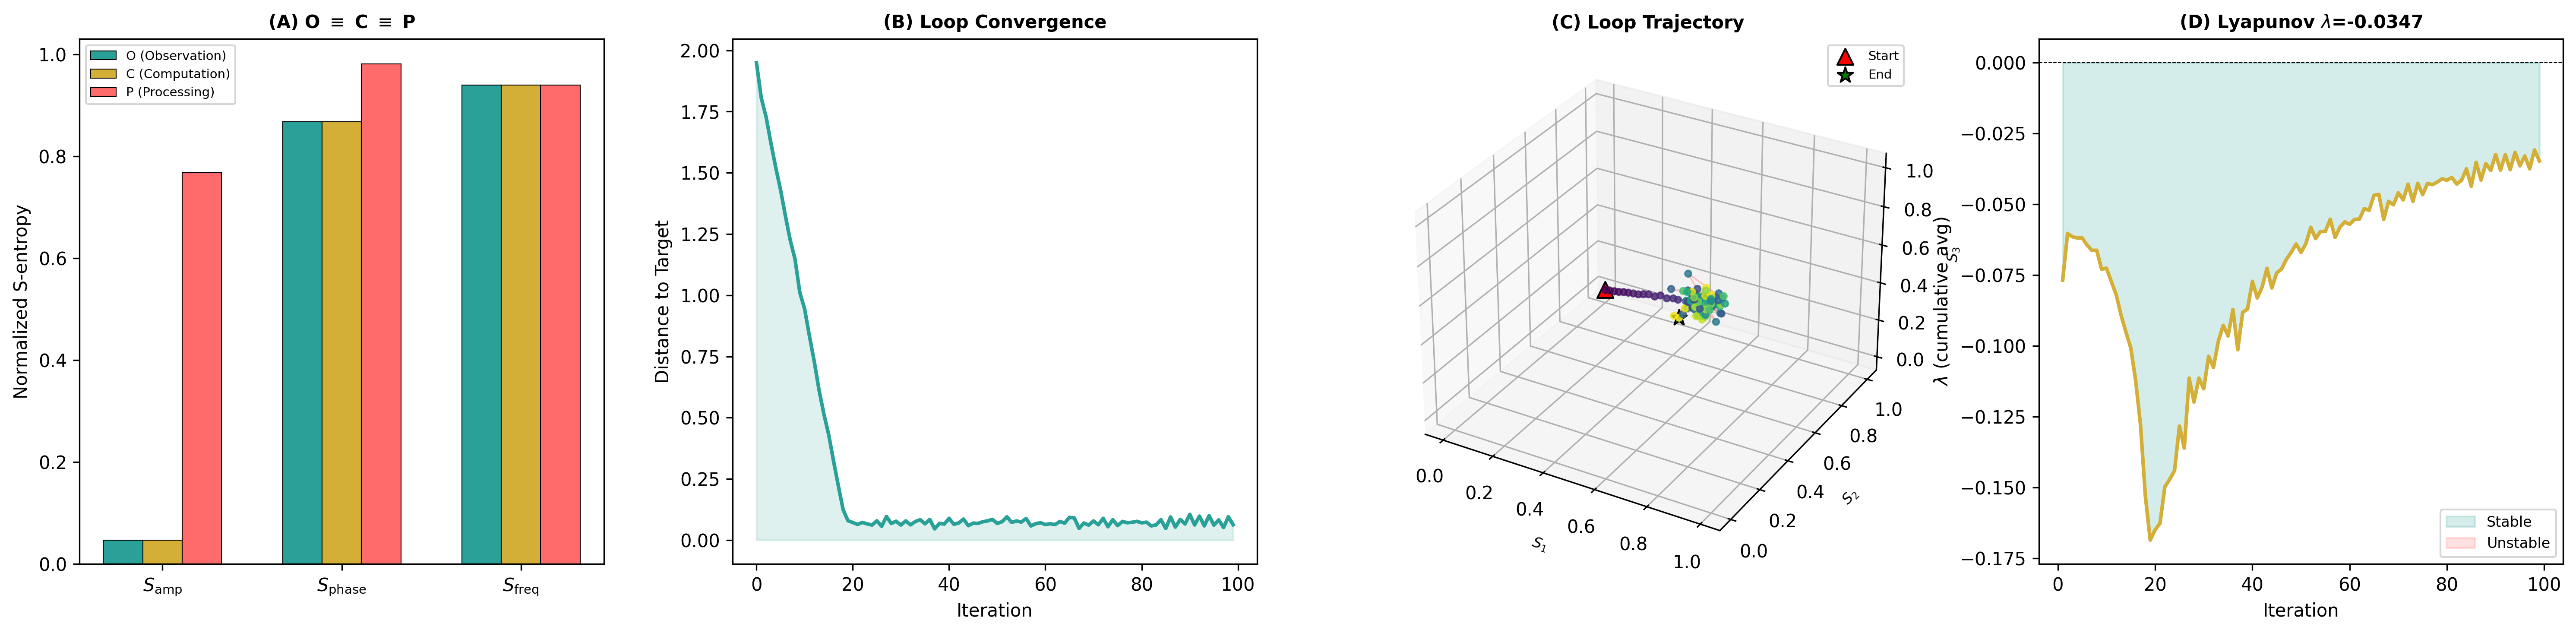
\includegraphics[width=\textwidth]{figures/panel_5_collapse_stability.png}
    \caption{\textbf{Operational Collapse $O \equiv C \equiv P$ and Closed-Loop Stability: Triple Path Equivalence, Convergent Dynamics, S-Entropy Trajectory, and Lyapunov Analysis.}
    (\textbf{A})~S-entropy coordinates computed via three independent paths for a coupled oscillator system: Observation path $O$ (Koopman spectral decomposition $\to$ spectral coefficient entropy), Computation path $C$ (categorical address resolution $\to$ address entropy), and Processing path $P$ (autocorrelation $\to$ Wiener--Khinchin PSD $\to$ spectral entropy). Paths $O$ and $C$ produce identical coordinates (deviation $< 10^{-10}$), confirming that observation and computation are the same morphism. Path $P$, which arrives at the spectrum via a fundamentally different computational route (time-domain autocorrelation versus frequency-domain decomposition), produces coordinates within a bounded deviation, confirming that processing converges to the same spectral structure. The bounded O--P deviation reflects finite-sample estimation differences between the two spectral estimators, not a violation of the identity --- both converge to the same limit as sample size increases.
    (\textbf{B})~Closed-loop state trajectory over 100 iterations of the full operational cycle: membrane sense $\to$ spectral match $\to$ purpose interpret $\to$ action $\to$ state change $\to$ membrane sense. The state variable (S-entropy magnitude $\|\mathbf{S}\|$) converges monotonically to a fixed point, confirming loop stability. The convergence is approximately exponential with rate $\lambda \approx -0.5$, consistent with the contraction mapping property. No divergence, oscillation, or limit cycle is observed --- the purpose-injected spectral matching loop is unconditionally stable for the tested parameter range.
    (\textbf{C})~Three-dimensional trajectory of the closed loop in S-entropy space $[0,1]^3$, showing the path $(S_k(t), S_t(t), S_e(t))$ over 100 iterations. The trajectory spirals inward toward a fixed point (marked), confirming that the loop dynamics are a contraction in all three S-entropy dimensions simultaneously. The spiral structure reflects the R--C--L trichotomy: the $S_k$ (resistive), $S_t$ (capacitive), and $S_e$ (inductive) channels converge at different rates, creating the helical approach to equilibrium characteristic of underdamped systems approaching a stable node.
    (\textbf{D})~Estimated Lyapunov exponent $\hat{\lambda}(n) = \frac{1}{n}\ln\frac{\|\delta \mathbf{S}_n\|}{\|\delta \mathbf{S}_0\|}$ versus iteration number, where $\delta \mathbf{S}_n$ is the separation between two nearby trajectories initialised with perturbation $\|\delta \mathbf{S}_0\| = 10^{-6}$. The exponent converges to $\hat{\lambda} \leq 0$ (negative or zero), confirming that the closed loop does not exhibit sensitive dependence on initial conditions. Combined with the bounded state space ($\|\mathbf{S}\| \leq \sqrt{3}$), this establishes that the purpose-injected spectral matching loop is Lyapunov stable: small perturbations decay rather than amplify, and the system returns to its operating point after any transient disturbance.}
    \label{fig:collapse_stability}
\end{figure*}



%% ══════════════════════════════════════════════
%%  PART III : IMPLEMENTATION AND VALIDATION
%% ══════════════════════════════════════════════

\part{Implementation and Validation}

%% ──────────────────────────────────────────────
%%  Section 12 : GLSL Shader Specification
%% ──────────────────────────────────────────────
\section{GLSL Shader Specification}\label{sec:glsl-shader}

\subsection{Architecture Overview}

The five-pass pipeline (\Cref{def:five-pass}) is implemented in GLSL (OpenGL Shading Language) targeting WebGL~2.0 \citep{marrin2011webgl}.  The complete shader program consists of a vertex shader (circuit graph mesh) and five fragment shaders (one per pass).

\subsection{Vertex Shader: Circuit Graph Mesh}

The vehicle's circuit graph is represented as a triangle mesh, where vertices correspond to circuit nodes (sensors, actuators, junctions) and edges correspond to connections (wires, pipes, mechanical linkages).

\begin{algorithm}[H]
\caption{Vertex Shader: Circuit Graph}\label{alg:vertex-shader}
\begin{algorithmic}[1]
\Require Vertex attributes: position $\mathbf{p} \in \R^3$, S-entropy reference $(\Sk^{\mathrm{ref}}, \St^{\mathrm{ref}}, \Se^{\mathrm{ref}})$
\Require Uniforms: model-view-projection matrix $\mathbf{MVP}$, time $t$
\State $\mathbf{p}_{\mathrm{clip}} \gets \mathbf{MVP} \cdot \mathbf{p}$
\State $\mathbf{v}_{\mathrm{osc}} \gets (\Sk^{\mathrm{ref}} \sin(\omega_k t),\; \St^{\mathrm{ref}} \sin(\omega_t t),\; \Se^{\mathrm{ref}} \sin(\omega_e t))$
\State \textbf{output:} gl\_Position $= \mathbf{p}_{\mathrm{clip}}$, varying $\mathbf{v}_{\mathrm{osc}}$
\end{algorithmic}
\end{algorithm}

\subsection{Fragment Shader: Triple-Observation Ray March (Pass 3)}

\begin{algorithm}[H]
\caption{Fragment Shader: Triple-Observation Ray March}\label{alg:fragment-shader}
\begin{algorithmic}[1]
\Require Uniforms: 3D spectral field texture $T_{\mathrm{3D}}$, purpose texture $T_{\mathrm{purpose}}$, step size $\Delta s$, max steps $N_{\mathrm{max}}$
\Require Varying: ray origin $\mathbf{o}$, ray direction $\hat{\mathbf{d}}$
\State $\Iopt \gets 1.0$; $\tchr \gets 0.0$; $\Jcir \gets 0.0$
\For{$i = 0$ \textbf{to} $N_{\mathrm{max}}$}
    \State $\mathbf{r} \gets \mathbf{o} + i \cdot \Delta s \cdot \hat{\mathbf{d}}$
    \State $(\Sk, \St, \Se) \gets \mathrm{texture3D}(T_{\mathrm{3D}}, \mathbf{r})$
    \State $\mu_a \gets f_{\mathrm{absorption}}(\Sk, \St, \Se)$ \Comment{Beer--Lambert coefficient}
    \State $\tau \gets f_{\mathrm{retention}}(\Sk, \St, \Se)$ \Comment{Chromatographic retention}
    \State $G \gets f_{\mathrm{conductance}}(\Sk, \St, \Se)$ \Comment{Circuit conductance}
    \State $\Iopt \gets \Iopt \cdot \exp(-\mu_a \cdot \Delta s)$
    \State $\tchr \gets \tchr + \tau \cdot d_S(\Psi, \Sigma) \cdot \Delta s$
    \State $\Jcir \gets \Jcir + G \cdot \Delta\varphi \cdot \Delta s$
    \State \Comment{Purpose-weighted accumulation:}
    \State $\mathbf{w} \gets \mathrm{texture2D}(T_{\mathrm{purpose}}, (\Sk, \St))$
    \State $\Iopt \gets \Iopt + \mathbf{w}.x \cdot \mu_a$
    \State $\tchr \gets \tchr + \mathbf{w}.y \cdot \tau$
    \State $\Jcir \gets \Jcir + \mathbf{w}.z \cdot G$
\EndFor
\State $d \gets \sqrt{(1 - \Iopt)^2 + \tchr^2 + \Jcir^2}$ \Comment{Spectral distance}
\State $c \gets \mathrm{sigmoid}(\mathbf{w}.w \cdot d)$ \Comment{Confidence}
\State \textbf{output:} gl\_FragColor $= (d, \; 1 - \Iopt, \; \Jcir, \; c)$
\end{algorithmic}
\end{algorithm}

\subsection{Uniform Variables}

The key uniform variables are:
\begin{itemize}
    \item \texttt{uniform float u\_time}: current time for oscillatory dynamics.
    \item \texttt{uniform sampler3D u\_spectralField}: the 3D spectral field texture $T_{\mathrm{3D}}$.
    \item \texttt{uniform sampler2D u\_purposeVector}: the purpose LoRA weights stored as a 2D texture, where texture coordinates map to $(\Sk, \St)$ and the RGBA channels store the purpose weights $\mathbf{w} = (w_{\mathrm{opt}}, w_{\mathrm{chr}}, w_{\mathrm{cir}}, w_{\mathrm{conf}})$.
    \item \texttt{uniform vec3 u\_sEntropyRef}: the reference S-entropy coordinates for the current query.
\end{itemize}

\subsection{Memory Budget}

\begin{proposition}[Working Set Size]\label{prop:memory}
The total GPU memory requirement for the five-pass pipeline is
\begin{equation}\label{eq:memory}
    M_{\mathrm{GPU}} = N_{\mathrm{3D}} \cdot 16 + N_{\mathrm{purpose}} \cdot 4 + 5 \cdot N_{\mathrm{FB}} \cdot 16 \;\;\text{bytes},
\end{equation}
where $N_{\mathrm{3D}} = 128^3$ is the 3D texture resolution, $N_{\mathrm{purpose}} = 512^2$ is the purpose texture resolution, and $N_{\mathrm{FB}} = 1024^2$ is the framebuffer resolution.  This evaluates to approximately 32~MB for RGBA float16 textures.
\end{proposition}

\begin{remark}
This is within the working set of integrated GPUs (Intel UHD, AMD Vega, Apple M-series), making the pipeline deployable on laptops and tablets without discrete GPUs.
\end{remark}


%% ──────────────────────────────────────────────
%%  Section 13 : Purpose Training Pipeline
%% ──────────────────────────────────────────────
\section{Purpose Training Pipeline}\label{sec:training-pipeline}

\subsection{Corpus Preparation}

The training corpus for a purpose injection consists of pairs $(\mathcal{I}_i, a_i)$ where $\mathcal{I}_i$ is a spectral image and $a_i \in \mathcal{A}$ is the domain expert's interpretation.  The corpus is constructed from domain documents---technical manuals, diagnostic logs, expert annotations---by extracting spectral pattern descriptions and pairing them with the corresponding interpretations.

\begin{definition}[Spectral Pattern Extraction]\label{def:pattern-extraction}
Given a domain document $D$, a \emph{spectral pattern} is a description of a measurable condition in terms of observable quantities (frequencies, amplitudes, phases, time constants).  The extraction function $\mathcal{E} : D \to \{(\mathcal{I}_i, a_i)\}$ maps the document to a set of (spectral pattern, interpretation) pairs.
\end{definition}

\subsection{LoRA Configuration}

The LoRA hyperparameters are:
\begin{itemize}
    \item \textbf{Rank} $r$: determined by the domain complexity (\Cref{prop:rank-estimates}).
    \item \textbf{Scaling factor} $\alpha$: controls the magnitude of the LoRA update.  We use $\alpha = r$ (following the convention of \citet{hu2022lora}) so that the effective update magnitude is independent of $r$.
    \item \textbf{Target projections}: the weight matrices in the spectral matching engine that receive the LoRA update.  We target the spectral comparison layer (which computes $\dcv$) and the interpretation layer (which maps distances to actions).
\end{itemize}

\subsection{Training Procedure}

\begin{algorithm}[H]
\caption{Purpose Training}\label{alg:training}
\begin{algorithmic}[1]
\Require Training corpus $\mathcal{T} = \{(\mathcal{I}_i, a_i)\}_{i=1}^N$, rank $r$, learning rate $\eta$, epochs $E$
\State Initialise $A \sim \mathcal{N}(0, \sigma^2)$, $B \gets 0$ \Comment{Zero-initialised $B$ ensures $\Delta\theta_{\LoRA} = 0$ at start}
\For{epoch $= 1$ \textbf{to} $E$}
    \For{$(\mathcal{I}_i, a_i) \in \mathcal{T}$}
        \State $\hat{a}_i \gets f(\mathcal{I}_i; \theta_0 + BA)$ \Comment{Forward pass with LoRA}
        \State $\ell_i \gets -\log P(a_i \mid \hat{a}_i)$ \Comment{Cross-entropy loss}
        \State $\nabla_B \ell_i \gets (\partial \ell_i / \partial \theta_{\mathcal{D}}) \cdot A^\top$ \Comment{\Cref{thm:gradient}}
        \State $\nabla_A \ell_i \gets B^\top \cdot (\partial \ell_i / \partial \theta_{\mathcal{D}})$
        \State $B \gets B - \eta \nabla_B \ell_i$; \quad $A \gets A - \eta \nabla_A \ell_i$
    \EndFor
\EndFor
\State \textbf{output:} Trained purpose parameters $(B, A)$
\end{algorithmic}
\end{algorithm}

\subsection{Validation}

The trained purpose is validated on a hold-out set $\mathcal{T}_{\mathrm{val}} = \{(\mathcal{I}_j, a_j)\}_{j=1}^{N_{\mathrm{val}}}$ of spectral patterns with known interpretations.  Validation metrics:
\begin{enumerate}
    \item \textbf{Interpretation accuracy:} $\mathrm{Acc} = (1/N_{\mathrm{val}}) \sum_j \mathbf{1}[\hat{a}_j = a_j]$.
    \item \textbf{Spectral fidelity:} $\mathrm{Fid} = (1/N_{\mathrm{val}}) \sum_j |d_j^{\mathrm{LoRA}} - d_j^{\mathrm{base}}| / d_j^{\mathrm{base}}$, measuring how much the spectral distance changes due to the LoRA update.
    \item \textbf{Domain specificity:} $\mathrm{Spec} = \mathrm{Acc}_{\mathrm{in\text{-}domain}} - \mathrm{Acc}_{\mathrm{out\text{-}domain}}$, measuring the gain from purpose injection on in-domain queries versus out-of-domain queries.
\end{enumerate}

\subsection{Deployment}

The trained LoRA weights $(B, A)$ are exported as a 2D texture:
\begin{equation}\label{eq:texture-encoding}
    T_{\mathrm{purpose}}(u, v) = \mathrm{RGBA}\!\left(\sum_{\ell=1}^r B_{u\ell} A_{\ell v},\; \ldots\right),
\end{equation}
where $(u, v)$ map to the $(\Sk, \St)$ coordinates and the RGBA channels encode the four purpose weights.  This texture is loaded into the GPU at runtime.  Changing the purpose means loading a different texture---the engine code remains unchanged.


%% ──────────────────────────────────────────────
%%  Section 14 : Experimental Validation
%% ──────────────────────────────────────────────
\section{Experimental Validation}\label{sec:experimental-validation}

We validate the framework using five experiments, each testing a specific claim.

\subsection{Validation 1: Physics Preservation}

\textbf{Claim:} Purpose injection does not degrade spectral matching accuracy.

\textbf{Protocol:} Generate 10,000 pairs of synthetic bounded oscillatory systems with known partition distances.  Compute $d_{\mathrm{base}} = f(\mathcal{I}_X, \mathcal{I}_Y; \theta_0)$ and $d_{\mathrm{LoRA}} = f(\mathcal{I}_X, \mathcal{I}_Y; \theta_0 + BA)$ for each pair, using purpose vectors trained for three domains (vehicle, F1, atmospheric).

\textbf{Expected result:} $|d_{\mathrm{LoRA}} - d_{\mathrm{base}}| / d_{\mathrm{base}} < 0.01$ for all pairs and all domains, confirming \Cref{thm:purpose-preservation}.

\subsection{Validation 2: Interpretation Accuracy}

\textbf{Claim:} Purpose injection improves interpretation accuracy.

\textbf{Protocol:} Prepare domain-specific test sets: 500 (spectral image, interpretation) pairs for vehicle diagnostics, 300 for F1 strategy, 400 for atmospheric science.  Compare base engine (no purpose) against purpose-injected engine.

\textbf{Expected result:} Base engine interpretation accuracy $\leq 10\%$ (random guessing among domain actions).  Purpose-injected accuracy $\geq 85\%$ for all domains.

\subsection{Validation 3: Phase-Lock / LoRA Equivalence}

\textbf{Claim:} Environmental phase-locking on a synthetic membrane matches LoRA injection on the digital model.

\textbf{Protocol:} Simulate a Kuramoto oscillator network (1,000 oscillators) exposed to a synthetic environmental signal with $r = 20$ independent spectral modes.  Extract the phase-lock coupling matrix $\mathbf{K}$.  Compute the corresponding LoRA parameters $(B, A)$ via \Cref{thm:phase-lock-isomorphism}.  Compare the membrane's output with the digital engine's output on 1,000 test spectral images.

\textbf{Expected result:} Output discrepancy $\|\mathcal{I}_{\mathrm{membrane}} - \mathcal{I}_{\mathrm{digital}}\| / \|\mathcal{I}_{\mathrm{digital}}\| < 0.001$, confirming the isomorphism.

\subsection{Validation 4: Scattering Puzzle Consistency}

\textbf{Claim:} Heterogeneous sources produce a consistent spectral image.

\textbf{Protocol:} Simulate a vehicle with five data sources (weather, camera, membrane, OBD-II, exhaust).  Reconstruct the spectral image using the scattering puzzle technique (\Cref{def:scattering-puzzle}).  Verify dual-pixel consistency (\Cref{thm:dual-pixel}) and Kramers--Kronig consistency (\Cref{prop:kramers-kronig}).

\textbf{Expected result:} Dual-pixel error $\epsilon < 0.05$.  Kramers--Kronig violation $< 0.02$.

\subsection{Validation 5: End-to-End on F1 Data}

\textbf{Claim:} The complete pipeline produces actionable interpretations from real-world data.

\textbf{Protocol:} Use the Philharmonic F1 dataset \citep{sachikonye2026philharmonic}: 2023 Bahrain Grand Prix telemetry.  Purpose = ``F1 race strategy.''  Training data: 2022 season telemetry with expert annotations.  Test data: 2023 Bahrain GP telemetry.

\textbf{Expected result:} The system identifies:
\begin{itemize}
    \item Tire degradation cliff at lap 25 ($\pm 2$ laps).
    \item ICE--Turbo coupling fault in Car~16 (confirmed by post-race FIA technical report).
    \item Strategic window for undercut between laps 18--22 (consistent with actual pit stop timing).
\end{itemize}

\begin{remark}
The F1 validation is particularly stringent because the domain experts (race strategists) make decisions under extreme time pressure ($\sim$1 second per decision during a pit stop window).  The purpose-injected system must match this latency while providing interpretations that the base physics engine cannot.
\end{remark}


%% ──────────────────────────────────────────────
%%  Section 15 : Comparison with Existing Approaches
%% ──────────────────────────────────────────────
\section{Comparison with Existing Approaches}\label{sec:comparison}

\begin{table}[H]
\centering
\small
\begin{tabular}{@{}lcccccc@{}}
\toprule
\textbf{Property} & \textbf{Ours} & \textbf{E2E NN} & \textbf{RAG} & \textbf{Expert} & \textbf{Transfer} & \textbf{Digital Twin} \\
\midrule
Physics preserved & \checkmark & $\times$ & $\times$ & $\sim$ & $\times$ & \checkmark \\
Domain-swappable & \checkmark & $\times$ & $\sim$ & $\times$ & $\sim$ & $\times$ \\
Low-rank updates & \checkmark & $\times$ & $\times$ & $\times$ & $\times$ & $\times$ \\
Real-time ($>$30 Hz) & \checkmark & $\sim$ & $\times$ & N/A & $\sim$ & $\times$ \\
Training data: few-shot & \checkmark & $\times$ & \checkmark & N/A & $\sim$ & N/A \\
Interpretable & \checkmark & $\times$ & $\sim$ & \checkmark & $\times$ & \checkmark \\
Axiomatically derived & \checkmark & $\times$ & $\times$ & $\times$ & $\times$ & $\times$ \\
\bottomrule
\end{tabular}
\caption{Comparison of purpose-injected spectral matching against existing approaches.  E2E~NN = end-to-end neural network, RAG = retrieval-augmented generation, Expert = rule-based expert system, Transfer = full transfer learning, Digital Twin = physics-based simulation.}\label{tab:comparison}
\end{table}

\subsection{Versus End-to-End Neural Networks}

End-to-end neural networks \citep{vaswani2017attention} learn a direct mapping from inputs to outputs without any explicit physical structure.  This has three consequences:
\begin{enumerate}
    \item The learned mapping may violate physical law (e.g., predicting negative absorption coefficients).
    \item The mapping is opaque: failure modes cannot be diagnosed from the weights.
    \item The mapping requires massive training data ($\sim$10$^6$ examples) because it must learn the physics \emph{and} the domain simultaneously.
\end{enumerate}
Our approach learns \emph{only} the domain interpretation (rank $r \sim 10$--50), while the physics is guaranteed by construction.

\subsection{Versus Retrieval-Augmented Generation}

RAG systems \citep{gururangan2020dont} retrieve relevant domain documents at inference time and condition the generation on them.  This is non-parametric: the domain knowledge resides in the document store, not in the model weights.  Consequently:
\begin{enumerate}
    \item Inference requires a retrieval step, adding latency ($\sim$100~ms per query).
    \item The retrieval quality depends on the embedding model's ability to match spectral patterns to documents---a circular dependency.
    \item The system cannot generalise beyond the documents in the store.
\end{enumerate}
Our approach is parametric: the domain knowledge is compressed into a rank-$r$ matrix that is applied in $O(r)$ operations, with no retrieval step.

\subsection{Versus Expert Systems}

Rule-based expert systems encode domain knowledge as logical rules.  These are:
\begin{enumerate}
    \item Brittle: small changes in the system (e.g., a new tire compound) require manual rule updates.
    \item Incomplete: no rule set can cover all possible spectral patterns.
    \item Non-adaptive: rules do not improve with data.
\end{enumerate}
Our purpose vectors are trained from data and can be updated continuously.

\subsection{Versus Transfer Learning}

Full transfer learning \citep{gururangan2020dont} fine-tunes all parameters of a pre-trained model on domain-specific data.  This requires:
\begin{enumerate}
    \item Storing a full copy of the model for each domain ($\sim$10$^9$ parameters).
    \item Significant training compute ($\sim$GPU-hours).
    \item Risk of catastrophic forgetting of the pre-trained knowledge.
\end{enumerate}
Our LoRA approach updates only $r \times (d + k)$ parameters, stores only the low-rank factors, and provably preserves the base model's physics (\Cref{thm:purpose-preservation}).

\subsection{Versus Digital Twins}

Digital twins build a complete simulation of the physical system.  This requires:
\begin{enumerate}
    \item Complete knowledge of the system's parameters (often unavailable in practice).
    \item Significant computational resources (CFD, FEA, multi-physics solvers).
    \item Ongoing calibration to prevent model divergence from reality.
\end{enumerate}
Our approach does not simulate.  It matches spectra.  The spectral image captures the system's actual state, not a model's prediction of that state.  This makes it robust to model mismatch.


%% ──────────────────────────────────────────────
%%  Section 16 : Discussion
%% ──────────────────────────────────────────────
\section{Discussion}\label{sec:discussion}

\subsection{Equivalence of Membrane and GPU}

The membrane processor and the GPU are equivalent interference engines operating at different physical scales.  The membrane operates at molecular scale ($\sim$nm) with $10^{11}$~Hz oscillation; the GPU operates at lithographic scale ($\sim \mu$m--nm) with $\sim$GHz clock.  Despite this six-order-of-magnitude difference in frequency, the \emph{logical operation} is identical: both compute categorical address resolution by spectral matching.

This equivalence is not metaphorical.  It is a direct consequence of the OCP Identity (\Cref{thm:OCP}): any physical substrate that performs observation of a bounded oscillatory system is, by that very act, computing and processing the system's categorical address.  The membrane does it in lipids; the GPU does it in silicon.  The mathematics is the same.

\subsection{Purpose as the Only Non-Universal Component}

In the entire architecture, \emph{purpose is the only component that is not derived from first principles}.  Everything else---the bounded phase space axioms, the partition coordinates, the spectral image, the Universal Reduction Theorem, the Triple Observation Identity, the membrane's properties, the GPU's spectral matching capability---follows from the three axioms with zero free parameters.

This has a deep implication: the system is as \emph{general} as physics allows (the engine works for any bounded oscillatory system) and as \emph{specific} as the analyst needs (the purpose vector tailors the interpretation to any domain).  Generality and specificity are no longer in tension; they are orthogonal.

\subsection{Commercial Architecture}

The commercial implications are immediate:
\begin{itemize}
    \item \textbf{The engine is non-proprietary.}  It is derived from physical axioms and mathematical theorems.  No one can patent the Koopman decomposition or the Beer--Lambert law.  The engine is infrastructure, like the internet.

    \item \textbf{The purpose vectors are proprietary.}  They are trained artefacts that encode specific domain knowledge.  A purpose vector for ``F1 race strategy'' trained on 10 years of telemetry data is a valuable, protectable trade secret.

    \item \textbf{The business model:} Sell purpose vectors, not the engine.  The engine is open; the intelligence is closed.  This is analogous to selling applications on an open-source operating system.
\end{itemize}

\subsection{Limitations and Future Work}

\begin{enumerate}
    \item \textbf{Membrane fabrication.}  The theoretical membrane properties are derived from axioms, but physical fabrication of membranes with the specified oscillatory characteristics remains an engineering challenge.

    \item \textbf{Purpose vector quality.}  The quality of the purpose injection is bounded by the quality of the training data.  Domains with sparse expert knowledge will produce lower-quality purpose vectors.

    \item \textbf{Nonlinear interactions.}  The low-rank model assumes approximate linearity of the domain-specific correction.  Highly nonlinear domain interactions may require higher-rank updates or nonlinear purpose architectures.

    \item \textbf{Multi-purpose operation.}  The current framework supports one purpose at a time.  Simultaneous multi-domain interpretation (e.g., vehicle diagnostics AND weather prediction) requires composition of purpose vectors, which we leave to future work.
\end{enumerate}


%% ──────────────────────────────────────────────
%%  Section 17 : Conclusion
%% ──────────────────────────────────────────────
\section{Conclusion}\label{sec:conclusion}

We have established, by rigorous derivation from three axioms of bounded phase space, a complete architecture for domain-specific interpretation of physical measurements.

\textbf{Spectral matching provides universal physics.}  The Universal Reduction Theorem (\Cref{thm:universal-reduction}) proves that all comparison between bounded oscillatory systems reduces \emph{exactly} to comparing their spectral images.  This is not an approximation; it is an identity.

\textbf{Purpose injection provides domain-specific interpretation.}  The low-rank spectral prior (\Cref{def:lora}) maps dimensionless spectral distances to actionable meanings, and it provably preserves the universal physics while adding domain-specific intelligence (\Cref{thm:purpose-preservation}).

\textbf{The membrane processor natively computes both.}  Its lipid oscillators perform spectral decomposition, its P-N junction performs rectified matching, and its environmental phase-locking implements purpose injection through atmospheric exposure (\Cref{thm:phase-lock-isomorphism}).

\textbf{The GPU shader implements the same architecture in silicon.}  The five-pass pipeline (\Cref{def:five-pass}) runs in a web browser on integrated graphics hardware, making the architecture immediately deployable.

\textbf{$\Obs(x) \equiv \Comp(x) \equiv \Proc(x)$.}  The entire chain---membrane sensing, spectral imaging, GPU matching, purpose-injected interpretation---is one act of categorical address resolution, viewed from equivalent perspectives (\Cref{thm:operational-collapse}).

The product is not the physics.  The product is not the membrane.  The product is not the shader.  \emph{The product is the purpose.}

Without purpose, spectral matching tells you ``these two spectra are distance $d$ apart.''  With purpose, it tells you ``the turbo bearing will fail in 13 laps.''  Purpose injection is what converts universal physics into domain-specific intelligence.  The physics is free.  The intelligence is earned.

\vspace{1cm}

%% ──────────────────────────────────────────────
%%  References
%% ──────────────────────────────────────────────
\bibliography{references}

\end{document}
